%\documentclass[12pt,letterpaper,twoside]{report}
\documentclass[12pt,letterpaper]{report}
\linespread{1.67} % Linespacing for entire thesis
% Standard packages
\usepackage{graphicx} % PostScript figures
\usepackage[centertags,fleqn]{amsmath}
\usepackage{amsfonts} 
\usepackage{amsbsy}
\usepackage{amssymb}
\usepackage{subfig}
\usepackage{caption}
\usepackage{amsthm,amstext}
\usepackage{newlfont} 
%\usepackage[hang]{subfigure} \usepackage{portland}
\usepackage{multirow}
\usepackage{verbatim}
\usepackage{url}
\usepackage{euscript}
\usepackage{algorithmic}
%\usepackage{dashbox}
\usepackage{setspace} % 1.5 spacing
\usepackage{longtable}
\usepackage[fancyhdr]{UMCCsThesis} % Thesis style
\usepackage{color}
\usepackage{float}
\floatstyle{ruled}
%\newfloat{algorithm}{htbp}{loa}
%\floatname{algorithm}{Algorithm}
\usepackage{upgreek,fontenc}
\usepackage[retainorgcmds]{IEEEtrantools}

%\usepackage{parsetree}

\hyphenpenalty=100
\tolerance=5000


% Defines name, thesis title, etc.
\usepackage{myowndef}
\DeclareMathOperator{\CU}{CU}
\DeclareMathOperator{\GCU}{GenCU}
\newcommand{\gaussN}[1]{\mathcal{N}\left\{#1\right\}}
\newcommand{\m}[1]{\mathbf{#1}}
\renewcommand{\v}[1]{\mathbf{#1}}
\newcommand{\ea}{\tilde{\mathbf{m}}}

\newtheoremstyle{example}{\topsep}{\topsep}%
    {}%           Body font
    {}%           Indent amount (empty = no indent, \parindent = para indent)
    {\bfseries}%  Thm head font
    {}%           Punctuation after thm head
    {\newline}%   Space after thm head (\newline = linebreak)
    {\thmname{#1}\thmnumber{ #2}\thmnote{ #3}}%         Thm head spec

    \theoremstyle{example}
    \newtheorem{example}{Example}[section]



%Define some commonly used macros here
\newcommand{\nl}{\newline\indent} 
\renewcommand{\algorithmiccomment}[1]{ //\texttt{#1}}
\newcommand{\ac}{\algorithmiccomment}
\def\headrulehook{\color{black}} % Color the header rule

% Line spacing -----------------------------------------------------------
\newlength{\defbaselineskip}
\setlength{\defbaselineskip}{\baselineskip}
\newcommand{\setlinespacing}[1]%
           {\setlength{\baselineskip}{#1 \defbaselineskip}}
\renewcommand{\doublespacing}{\setlength{\baselineskip}%
                           {1.0 \defbaselineskip}}
\renewcommand{\singlespacing}{\setlength{\baselineskip}{\defbaselineskip}}

%========= Document start
\begin {document}
% Title pages
\title{\maintitle}
\thispagestyle{empty}
\vskip 10mm
\smalltitle
\vskip 10mm
\centerline{\rule{150mm}{0.2mm}}
\vskip 10mm
\centerline{A Thesis presented to the Faculty of the Graduate School}
\centerline{University of Missouri---Columbia}
\vspace{10mm}
\centerline{\rule{150mm}{0.2mm}}
\vspace{10mm}
\centerline{In Partial Fulfillment}
\centerline{of the Requirements for the Degree}
\centerline{of \fulldegree}
\vspace{10mm}
\centerline{\rule{150mm}{0.2mm}}
\vspace{10mm}
\centerline{by}
\vskip 4mm
\centerline{\MYNAME}
\vskip 4mm
\centerline{\myadvisor,\hspace{1mm} Thesis Supervisor}
\vskip 4mm 
\centerline{\defensedate}
\newpage

\thispagestyle{empty}
\vspace*{15cm}
\begin{center}
$\mbox{\copyright}$ copyright by \myname~ \defenseyear\\
All Rights Reserved
\end{center}
\newpage

\thispagestyle{empty}
The undersigned, appointed by the Dean of the Graduate School, have 
examined the thesis entitled:\par
\vskip 5mm
\smalltitle
\vskip5mm
presented by \myname \par
a candidate for the degree of \fulldegree \par
and hereby certify that in their opinion it is worthy of acceptance.
%\vskip 15mm
\vskip 15mm
\centerline{\rule{100mm}{0.2mm}}
\centerline{\myadvisor}%\vskip 12mm
\vskip 10mm
\centerline{\rule{100mm}{0.2mm}}
\secondreader%\vskip 12mm
\vskip 10mm
\centerline{\rule{100mm}{0.2mm}}
\thirdreader%\vskip 12mm
%\vskip 4mm
%\centerline{\rule{100mm}{0.2mm}}
%\fourthreader
\newpage


%\newpage
%\pagenumbering{roman}
%\setcounter{page}{2}
%\newpage
%\addcontentsline{toc}{chapter}{ACKNOWLEDGEMENTS}
%\vskip 10mm
%\centerline{\bf \large ACKNOWLEDGMENTS}
%\vskip 10mm
%\input{aknowledge}
%\newpage
%\addcontentsline{toc}{chapter}{ABSTRACT}
%\centerline {\large \bf ABSTRACT}
%\vskip 2mm 
 
%\newpage

%\thispagestyle{plain}
\section*{\centering Abstract}
\vspace{40pt}
\hspace{15pt}
\hspace{15pt} Examination of the behavior of Generalized Covariance Union (GCU) reveals a previously unsuspected superficial
relationship to the problem of finding a minimal enclosing ellipsoid of ellipsoids, also called a L\"owner ellipsoid. By
interpreting any mean and covariance pair of some estimate or measurement as the 1-$\sigma$ contour ellipsoid of its
associated Gaussian probability density function, the results of GCU appear to form a L\"owner 1-$\sigma$ ellipsoid
about the 1-$\sigma$ ellipsoids of its $n$ inputs. This thesis presents a means to analyze and test this behavior
numerically, detailing the one- and two-dimensional cases, using mathematics easily extensible into higher dimensions.
The current hypothesis, supported by experimental evidence, is that the relationship between GCU and the minimal
enclosing ellipsoid problem is one of equivalence. Subsequent to this finding, pending a formal proof, it will be
possible to apply tools from computational geometry to solve data fusion problems.


\thispagestyle{plain}


%===== Justification, spacing for the main text
%\raggedbottom

%========= Acknowledgments
\pagenumbering{roman}
\typeout{}
\setcounter{page}{2}
\addcontentsline{toc}{chapter}{Acknowledgments}
%\setcounter{page}{2} 
\section*{\centering Acknowledgments}
\hspace{15pt} I extend my greatest appreciation to my adviser, Dr. Jeffrey Uhlmann, for his constant support and
guidance. I thank him for his endless patience and dedication, without which this thesis could not have been realized.
He is the greatest mentor, teacher and friend, for which any student could ask. I also thank Dr. Simon Julier and Ottmar
Boschardt for their ideas and insight, which proved invaluable as this thesis progressed.
       


%========== Tables of contents, figures, tables
\tableofcontents
\setcounter{tocdepth}{3}
\newpage
\addcontentsline{toc}{chapter}{List of Figures}
\listoffigures
\newpage
\addcontentsline{toc}{chapter}{List of Tables}
\listoftables

%========= List of acronyms
%\newpage
%\typeout{}
%\clearpage
%\addcontentsline{toc}{chapter}{Acronyms}
%\include{chapters/acronyms}

%========= Definition of terms
%\newpage
%\typeout{}
%\clearpage
%\addcontentsline{toc}{chapter}{Definitions}
%\include{chapters/definitions}


%========== Abstract ==============
\newpage
\addcontentsline{toc}{chapter}{Abstract}
\typeout{}
\clearpage
\thispagestyle{plain}
\section*{\centering Abstract}
\vspace{40pt}
\hspace{15pt}
\hspace{15pt} Examination of the behavior of Generalized Covariance Union (GCU) reveals a previously unsuspected superficial
relationship to the problem of finding a minimal enclosing ellipsoid of ellipsoids, also called a L\"owner ellipsoid. By
interpreting any mean and covariance pair of some estimate or measurement as the 1-$\sigma$ contour ellipsoid of its
associated Gaussian probability density function, the results of GCU appear to form a L\"owner 1-$\sigma$ ellipsoid
about the 1-$\sigma$ ellipsoids of its $n$ inputs. This thesis presents a means to analyze and test this behavior
numerically, detailing the one- and two-dimensional cases, using mathematics easily extensible into higher dimensions.
The current hypothesis, supported by experimental evidence, is that the relationship between GCU and the minimal
enclosing ellipsoid problem is one of equivalence. Subsequent to this finding, pending a formal proof, it will be
possible to apply tools from computational geometry to solve data fusion problems.


\thispagestyle{plain}



%========= Main Body ==============
\cleardoublepage
\pagenumbering{arabic}

\typeout{}
\chapter{Introduction}\label{chapter:introduction}

\section{Background Information}

\PARstart{O}{ver} the last decade, Level-1 information management has matured significantly, with the development of
rigorous algorithms robust to the effects of unmodeled correlations, and corrupt and/or spurious information, in the
context of general distributed data fusion networks. Recent inroads into the development of higher level information
management applications have yielded significant improvements to the data fusion tool called Covariance Union
(CU)~\cite{uhlmann03,julier05}. CU is used to find the union of a set of input modes or state estimates in a way that
guarantees an accurate representation of the system's true state in circumstances when other tools may not; simply put,
it is a method to reduce many modes to one.

A higher level data fusion application is likely manage information in a multimodal scheme, using either Multi
Hypothesis Tracking (MHT) or a Gaussian Mixture Model (GMM). MHT maintains multiple location and uncertainly estimates
corresponding to distinct possible states~\cite{barshalom88}. GMM is a parametrization of the Probability Density
Function (PDF) that describes the uncertainty distribution across the application. Since PDF approximations typically
only represent the significant modes of the distribution in terms of their mean and covariance, the representation
differs from that of MHT only in that a GMM interprets each mode as an explicit Gaussian PDF~\cite{fusion06}. Since
the implementation of these two techniques is identical, this thesis will use the GMM convention, of the form
  \begin{equation}\label{eqn:gmm}
    p(\mathbf{x})=\sum_{i=1}^Np_i\gaussN{\mathbf{x};\mu{_i},\sigma_i\sigma_i^T},
  \end{equation}
whenever referring to a multimodal state estimate, with the understanding that a Gaussian MHT model will be equivalent.

The fusion of a set $S$ of location and uncertainty estimates---each defining a possible state of the target, only one
of which is guaranteed to be consistent---with another set $T$ can be accomplished simply by forming the Cartesian
product $S\times T$ and applying the appropriate fusion algorithm (Kalman or Covariance Intersection) to the pairs.
Unfortunately, this yields a combined estimate that has $O(|S|*|T|)$ modes, which implies that the complexity of the
fused estimate exceeds that of the original estimates. This increasing complexity will tend to exhaust available
resources and therefore must be mitigated. CU can be used to combine modes, instead of pruning those deemed unnecessary
by some metric, and therefore reduce the information complexity of the fused set in a way that correctly estimates the
cumulative effect of the remaining modes~\cite{fusion06}.

\section{Notation}

Determining how to represent information and uncertainty, in either a single-target application or a multimodal system,
is a key first step that impacts all aspects of the data fusion problem. The representation must provide both an
estimate of the state of the target or system of interest {\em and} its associated degree of error or uncertainty, and
the uncertainty must be defined in a form that permits it to be empirically determined. There must be a rigorous
algorithm for fusing information in the representation, and the computational complexity of the representation and its
associated fusion algorithms must be bounded for practical application~\cite{fusion06}.

By far the most widely used information representation is the mean and covariance form, where the mean vector defines
the best estimate of the state of the target and the error covariance provides an upper bound on the expected squared
error associated with the mean. For example, the measured position of an object in two dimensions can be represented as
a vector $\v{m}$ consisting of the object's estimated mean position, e.g., $\v{m} = [x,y]^T$, and an
error covariance matrix $\m{M}$ that expresses the uncertainty associated with the estimated mean.  If the error in
the estimated mean vector is denoted as $\ea$, then the error covariance matrix is an estimate of the expected squared
error, E$[\ea\ea^T]$. The estimate is said to be {\em consistent} (or conservative) if and only if $\m{M}$ $\geq$
E$[\ea\ea^T]$ or, equivalently, $\m{M}$ - E$[\ea\ea^T]$ is positive definite or semidefinite (i.e., has no negative
eigenvalues). The full estimate of a target's state is given by the mean and covariance pair
$(\v{m},\m{M})$~\cite{fusion06,uhlmann03}. Although the GMM convention explicitly defines its own notation, as in
equation \ref{eqn:gmm}, the mean and covariance notation will be used throughout this thesis whenever referring to any
probabilistic estimate.


\section{Problem Definition}

Generalized Covariance Union (GCU) forms an important part of the hierarchy of data fusion tools which includes the
Kalman filter, Covariance Intersection, and the optimal form of CU. Each of these tools is capable of generating a
consistent result over a set of $n$ input estimates $(\v{m}_i,\m{M}_i)$, given certain preconditions. However, practical
running times for the current implementation of CU and GCU prohibit the use of these tools in any real-time
applications (operational cost is roughly proportional to the number of estimates $n$, and the cube of the
dimensionality of the state space)~\cite{fusion06}.

Research into GCU has revealed a remarkable superficial similarity to the problem of finding a Minimal Enclosing
Ellipsoid of Ellipsoids (MEEE), a common technique from computational geometry and computer graphics. These two problems
are very different, in the sense that mean and covariance estimates in tracking and data fusion refer to moments of a
possibly unknown underlying probability distribution, whereas ellipsoidal intersection and containment involves finite
volumes of space. Despite any differences between GCU and MEEE in representation and formulation, the similarities
between the results are suggestive of some level of equivalence.

This thesis will examine the GCU optimization problem and the possible applicability of techniques from computational
geometry, by presenting evidence that GCU and MEEE techniques may in fact be used to solve the same problem.


\section{Organization of Thesis}


The organization of this thesis is outlined as follows. Chapter \ref{chapter:introduction} begins by providing background
information and motivation for the research proposed in this thesis. A definition of the problem is given next, to
outline the scope of the research.

Work leading up to the research presented here is detailed in Chapter \ref{chapter:gcu}. This chapter will present the
Kalman filter, Covariance Intersection, and Covariance Union as part of a framework of data fusion tools. Generalized
Covariance Union is presented here as well, after this framework has been established.

Chapter \ref{chapter:meee} will define the problem of finding a Minimal Enclosing Ellipsoid of Ellipsoids, and give a
method to test whether a proposed enclosing ellipsoid properly contains its enclosed ellipsoids, as it should. Also given
in this chapter is a transformation between mean-covariance space and ellipsoid space, in order to provide a way for the
GCU and MEEE results to be compared.

Chapter \ref{chapter:analysis} will present the results of this research, experimental evidence and mathematical
analysis that demonstrate the relationship between GCU and MEEE.

This thesis concludes with a summary of accomplishments and dialog for future work in Chapter
\ref{chapter:conclusion}.





\typeout{}
\chapter{Generalized Covariance Union}\label{chapter:gcu}

\section{Data Fusion Framework}\label{section:framework}

\PARstart{C}{ovariance Union}, in both its Optimal and Generalized forms, is part of a larger hierarchy of data fusion
tools which when used properly together cover a broad range of possible situations, and form a robust framework with
which to build higher-level applications~\cite{fusion06,uhlmann03}. The remainder of this section is given to present
the previously published portions of this framework, the Kalman filter, Covariance Intersection, and Optimal Covariance
Union; both as background information and to provide the proper context for Generalized Covariance Union, which is 
detailed in sections \ref{section:motivation} and \ref{section:gcu}.


% SECTION Kalman
\subsection{Kalman Filter}

The most basic concept of data fusion is the idea that two pieces of information can be ``fused'' to create
a new piece of information which is ``better'' than the two inputs by some metric. One tool used to perform this action
is the Kalman filter. The Kalman filter addresses the general problem of trying to estimate the state $\v{x}\in\Re$  of
a discrete-time controlled process that is governed by the linear stochastic difference equation
\begin{equation}\label{eqn:kalsto}
    \v{x}_k = \m{A}\v{x}_{k-1} + \m{B}\v{u}_k + \v{w}_{k-1} ,
\end{equation}
with a measurement $\v{z}\in\Re$ that is
\begin{equation}\label{eqn:kalmeasure}
\v{z}_k = \m{H}\v{x}_k + \v{v}_k.
\end{equation}
where $\v{w}_k$ and $\v{v}_k$ are random variables which represent the process and measurement noise, respectively,
where $\m{H}_i$ is the transformation for the state space of the fused estimate to the state space of the
estimate~\cite{siggraph01}.

The filter operates in two steps for every discrete unit of time. The first step is the projection step, in which the 
future state of a system is estimated, projecting forward from time step $k-1$ to the current time step $k$. This is 
given by
\begin{align}
    \v{x}^-_k &= \m{A}\v{x}_{k-1}+\m{B}\v{u}_k\\
    \m{P}^-_k &= \m{A}\m{P}_{k-1}\m{A}^T+\m{Q}
\end{align}
where $\m{Q}$ is the process noise covariance defining the PDF for the variable $\v{w}_k$ from equation \ref{eqn:kalsto}.
The second step is the update step, in which the actual measurements are used to correct the predicted state. This is
given by
\begin{align}
    \v{x}_k &= \v{x}^-_k+\m{K}_k(\v{z}_k-\m{H}\v{x}^-_k)\\
    \m{P}_k &= (\m{I}-\m{K}_k\m{H})\m{P}^-_k,\\
\intertext{with}
    \m{K}_k &= \m{P}^-_k\m{H}^T(\m{H}\m{P}^-_k\m{H}^T+\m{R})^{-1},
\end{align}
where $\m{R}$ is the measurement noise covariance defining the PDF for the variable $\v{v}_k$ from equation
\ref{eqn:kalmeasure}~\cite{siggraph01}.

In addition to a time-sequence of measurements received from the same source, the Kalman filter may also be applied to a
set of separate measurements from different sources. Given a set of statistically {\em independent} (uncorrelated) estimates
$(\v{m}_1,\m{M}_1),(\v{m}_2,\m{M}_2),\dots,(\v{m}_n,\m{M}_n)$, the Kalman fusion equations can be written
as~\cite{uhlmann03,maybeck79}
\begin{figure}[tbp]
    \centering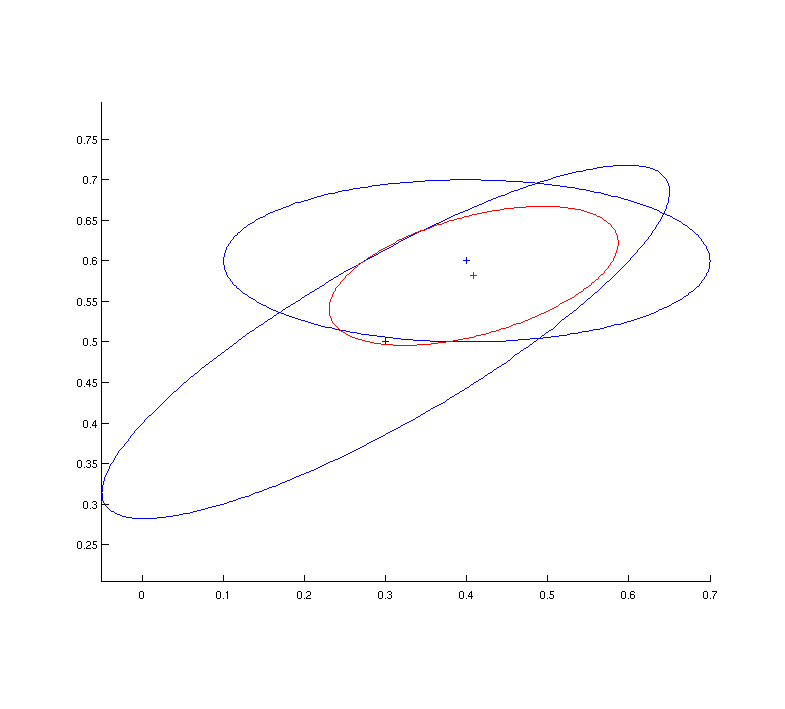
\includegraphics[width=0.6\textwidth]{figures/kalman2d.png}
    \caption{\it 1-$\sigma$ contour plots of two 2D inputs (blue) together with the Kalman fused result (red). Note that
        these contours are a distance of $\sigma$ away from the mean on a 2D Gaussian surface, and do not represent a
        closed volume or area. }
    \label{fig:kalman2d}
\end{figure}
\begin{align}
    \m{C} &= (\m{M}^{-1}_1+\m{M}^{-1}_2+\dots+\m{M}^{-1}_n)^{-1}\label{eqn:kalmanP}\\
    \v{c} &= \m{C}(\m{M}^{-1}_1\v{m}_1+\m{M}^{-1}_2\v{m}_2+\dots+\m{M}^{-1}_n\v{m}_n).\label{eqn:kalmanx}
\end{align}
Figure \ref{fig:kalman2d} illustrates the correct operation of the Kalman filter on two estimates known to be both
consistent and independent. Although the two input estimates and the fused Kalman result in the example are all 2D
Gaussian surfaces (which are greater than or equal to some unknown underlying PDF), it is convenient to represent these
probabilistic models simply by showing the 1-$\sigma$ contour centered at the mean.

In either form, the underlying assumptions in all Kalman applications are consistency and independence. However, any
presumption of statistical independence should be carefully considered, since virtually any sensor is subject to
time-correlated errors resulting from the particular conditions of its use; additionally errors associated with the 
non-linear transformation of its measurements are deterministic and therefore non-independent~\cite{uhlmann03}. For
example, any changes in temperature, barometric pressure, or humidity which affect the operation of a sensor's internal
electronics, and their effect on the sensor's accuracy, must be known {\em exactly}, or the assumption of independence
does not hold.
\begin{figure}[tbp]
    \centering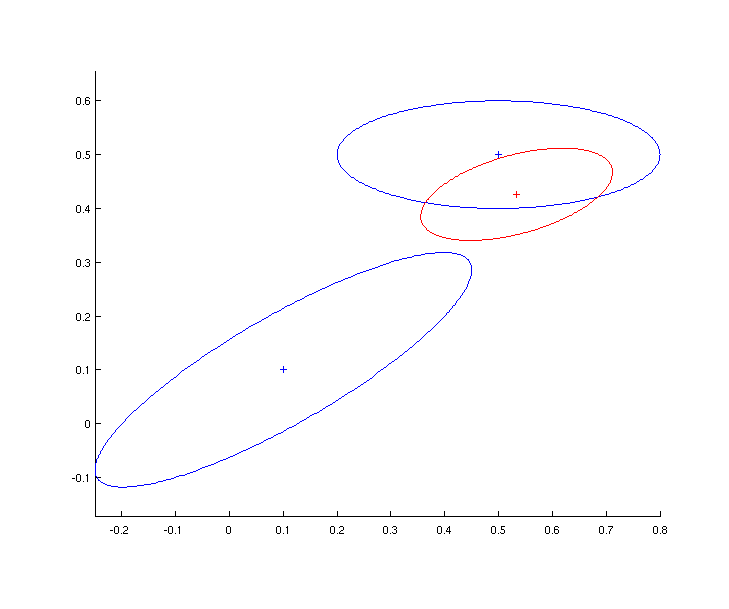
\includegraphics[width=0.6\textwidth]{figures/kalman2d-i.png}
    \caption{\it 1-$\sigma$ contour plots of two 2D inputs (blue) together with the Kalman fused result (red),
        illustrating a potentially inconsistent result. Note that the 1-$\sigma$ contours of the inputs, which are
        supposed to be independent estimates of the same position, do not overlap, suggesting that one may be the result
        of spurious data. One of the means is clear outlier when compared to the Kalman contour.}
    \label{fig:kalman2d-i}
\end{figure}
Figure \ref{fig:kalman2d-i} shows an example of what happens when the precondition for consistency is violated. The two
input estimates in this example are interpreted by the Kalman filter to be estimates of the same position, yet they are
far enough apart to suggest that one estimate might be the result of spurious data. Note that the 2D Gaussian surfaces
represented by the plotted 1-$\sigma$ contours do overlap, but not in the part of the surface that contains the highest
probability. The Kalman result shown will most likely not be consistent, but there is no way to correct for this
behavior.

To reiterate, the Kalman filter operates correctly if all its estimates are both consistent and independent.


% SECTION 1.2 CI
\subsection{Covariance Intersection}

Consider here the fusion of two estimates using either the Kalman filter or the data fusion technique known as
Covariance Intersection (CI), under the following circumstances:~\cite{uhlmann03}
\begin{enumerate}
\item {\em The two estimates are independent.} In this case the Kalman filter produces an optimal fused estimate while
CI produces a consistent, though suboptimal, estimate.
\item {\em The two estimates are completely correlated.} In this case CI produces an optimal fused estimate while
Kalman produces an inconsistent estimate.
\item {\em The two estimates are partially correlated.} In this case CI produces a consistent, though suboptimal,
estimate while the Kalman filter produces an inconsistent estimate.  \end{enumerate}
In each case, CI produces a consistent result, allowing it to operate safely in conditions which cause the Kalman filter
to fail.

The formulation of the CI equations follows from the joint covariance structure which exists between a given pair of
estimates $(\v{m}_1,\m{M}_1)$ and $(\v{m}_2,\m{M}_2)$
\begin{equation}\label{eqn:jointcov}
\left[\begin{array}{cc}
    \m{M}_1 & \m{X} \\
    \m{X}^T & \m{M}_2
\end{array}\right]
\end{equation}
where $\m{X}$ represents the actual, but unknown, cross covariance between the two estimates~\cite{uhlmann03}. Without
complete and exact knowledge of $\m{X}$, the only way to ensure consistency is to identify a joint covariance that is
guaranteed to be consistent based on the information available. This can be achieved by selecting a scalar value
$\omega, 0\leq1,$ and verifying that
\begin{equation}\label{eqn:cijointcov}
\left[\begin{array}{cc}
    \frac{1}{\omega}\m{M}_1 & 0 \\
    0                       & \frac{1}{1-\omega}\m{M}_2
\end{array}\right]
\leq
\left[\begin{array}{cc}
    \m{M}_1 & \m{X} \\
    \m{X}^T & \m{M}_2
\end{array}\right].
\end{equation}


This formulation of the $\omega$-parametrized covariance can be expanded from $2$ to $n$ estimates as follows
\begin{equation}\label{eqn:ncijointcov}
\left[\begin{array}{cccc}
    \omega_1\m{M}^{-1}_1 &                    0 &                    0 &                    0 \\
                       0 & \omega_2\m{M}^{-1}_2 &                    0 &                    0 \\
                       0 &                    0 &               \ddots &                    0 \\
                       0 &                    0 &                    0 & \omega_n\m{M}^{-1}_n
\end{array}\right],
\end{equation}
by selecting $\omega_1\dots\omega_n$ such that $1=\sum_{i=1}^n\omega_i$. By applying the inverse Kalman filter equations
\ref{eqn:kalmanP} and \ref{eqn:kalmanx} to \ref{eqn:ncijointcov}, the CI fusion equations for $n$ estimates with 
completely unknown degrees of correlation can be written as
\begin{figure}[tbp]
    \centering
        \subfloat[$\omega_1$=0.05]{\label{fig:ci2d05}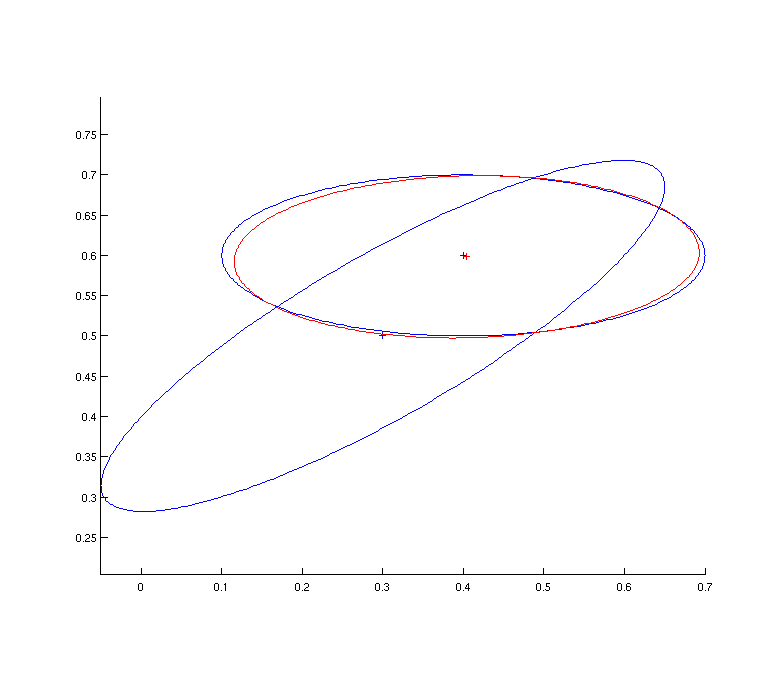
\includegraphics[width=0.4\textwidth]{figures/ci2d-05.png}}
        \subfloat[$\omega_1$=0.25]{\label{fig:ci2d25}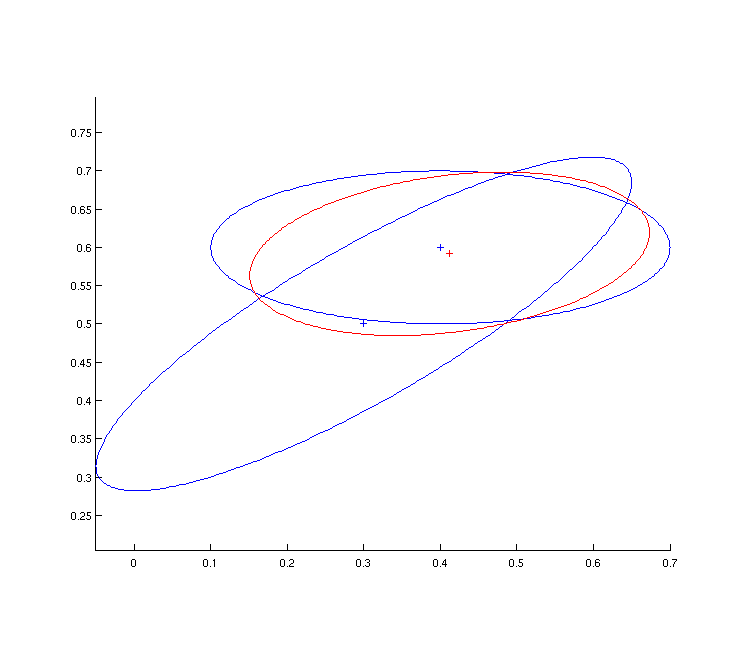
\includegraphics[width=0.4\textwidth]{figures/ci2d-25.png}}

        \subfloat[$\omega_1$=0.50]{\label{fig:ci2d50}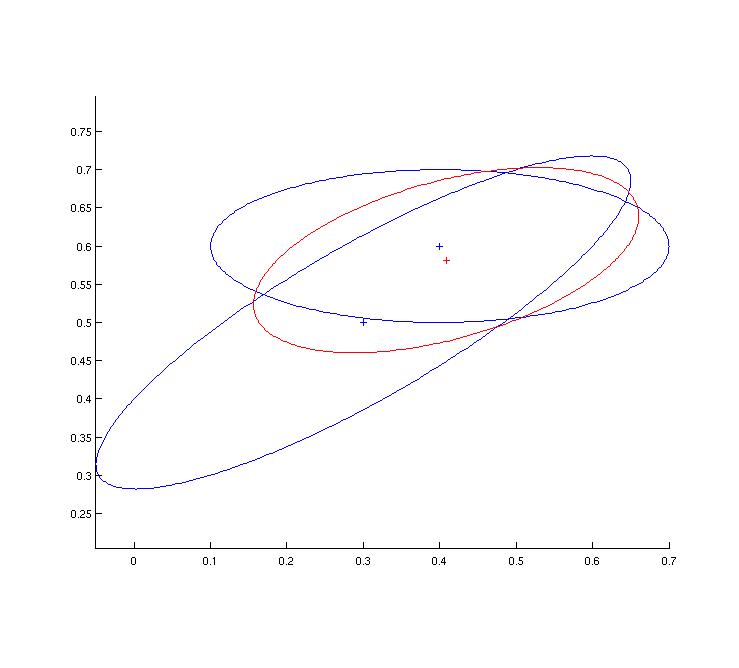
\includegraphics[width=0.4\textwidth]{figures/ci2d-50.png}}
        \subfloat[$\omega_1$=0.75]{\label{fig:ci2d75}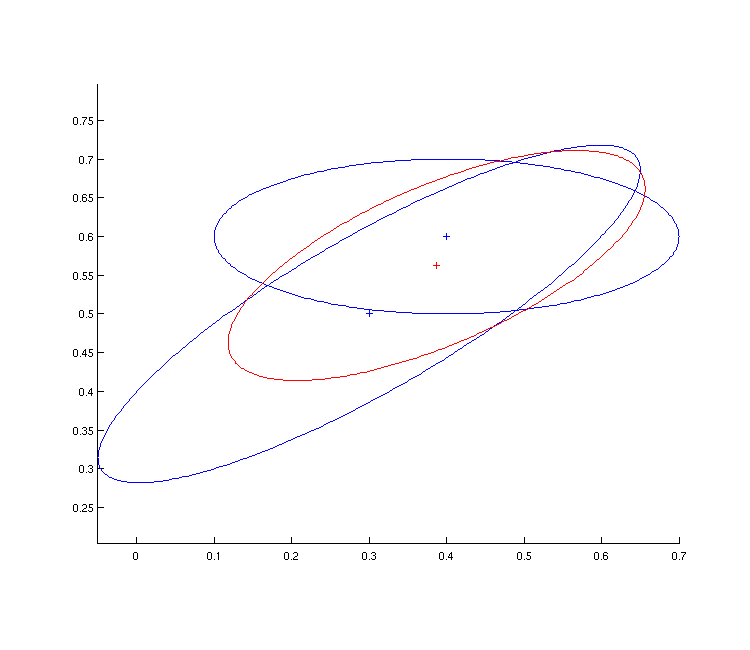
\includegraphics[width=0.4\textwidth]{figures/ci2d-75.png}}

        \subfloat[$\omega_1$=0.95]{\label{fig:ci2d95}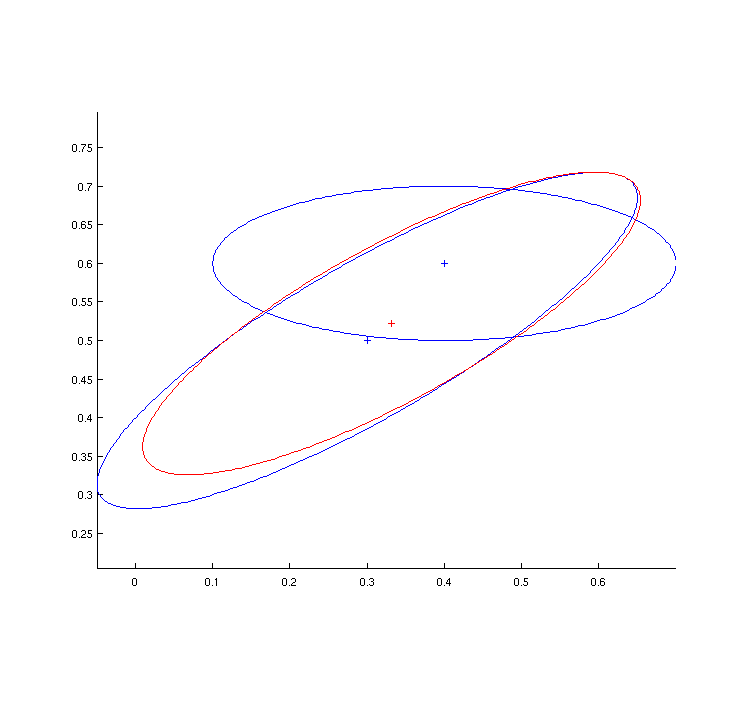
\includegraphics[width=0.4\textwidth]{figures/ci2d-95.png}}
    \caption{\it 1-$\sigma$ contour plots for two 2D input estimates (blue) together with the CI fused result (red), for
        different values of $\omega$. Note how the CI result contour behaves like an interpolation between these two
        inputs as $\omega$ varies from 0 to 1. }
    \label{fig:ci2d}
\end{figure}
\begin{align}
    \m{C} &= \left(\omega_1\m{H}_1^T\m{M}^{-1}_1\m{H}_1+\omega_2\m{H}_2^T\m{M}^{-1}_2\m{H}_2+\dots+\omega_n\m{H}_n^T\m{M}^{-1}_n\m{H}_n\right)\label{eqn:cicov}\\
    \v{c} &= \m{C}\left(\omega_1\m{H}_1^T\m{M}^{-1}_1\v{m}_1+\omega_2\m{H}_2^T\m{M}^{-1}_2\v{m}_2+\dots+\omega_n\m{H}_n^T\m{M}^{-1}_n\v{m}_n\right)\label{eqn:cimean}
\end{align}
where $\m{H}_i$ is the transformation for the state space of the fused estimate to the state space of the estimate $i$
\cite{uhlmann03,fusion01}.

Figure \ref{fig:ci2d} shows an example of CI performed on a set of two input estimates. Different CI results are shown
for different values of $\omega$ in the range $(0,1)$, and each possible result is numerically consistent. An application which
performs CI should select the appropriate $\omega$ to minimize the size, e.g. the determinant, of the fused
covariance~\cite{uhlmann03}.

To reiterate, CI requires that all of its inputs be consistent, but it will function correctly in the face of partially
or completely correlated input data \footnote{CI as described here finds the optimal fused result when the correlation
between its inputs is completely unknown; but another form of CI called Split CI is optimal when the degree of
correlation is partially known, and the estimates can be represented in split covariance form. See Appendix B
of~\cite{uhlmann03} for more information.}.



% SECTION 3 CU
\subsection{Optimal Covariance Union}\label{section:cu}

In order to develop a completely robust data fusion application, it may be necessary to handle possibly spurious
measurements prior to any data fusion being performed. If two given estimates $(\v{m}_1,\m{M}_1)$ and
$(\v{m}_2,\m{M}_2)$ are determined to be mutually inconsistent with each other, i.e. the difference between their means
is much larger than what can be expected based on their respective error covariance estimates, then using either the
Kalman filter or CI equations will yield an inconsistent fused result~\cite{uhlmann03}.

Computing the Mahalanobis distance between the two estimates,
\begin{equation}\label{eqn:mahalanobis}
(\v{m}_1-\v{m}_2)^T(\m{M}_1+\m{M}_2)^{-1}(\v{m}_1-\v{m}_2),
\end{equation}
is one method to detect statistically significant deviations between these estimates (for example, as in figure
\ref{fig:kalman2d-i}). If such a deviation is detected, it can be assumed one of the estimates is the result of
spurious measurements or corrupted data, but it may not be possible to detect which of the estimates is at
fault~\cite{uhlmann03}.

Covariance Union (CU) is a data fusion technique which can be used to resolve such a confliction by finding a union
estimate which is consistent with both (or all of) its inputs. This union $(\v{u},\m{U})$ is found by minimizing some
measure of $\m{U}$, e.g. the determinant, subject to the following constraints,
\begin{figure}[tbp]
    \centering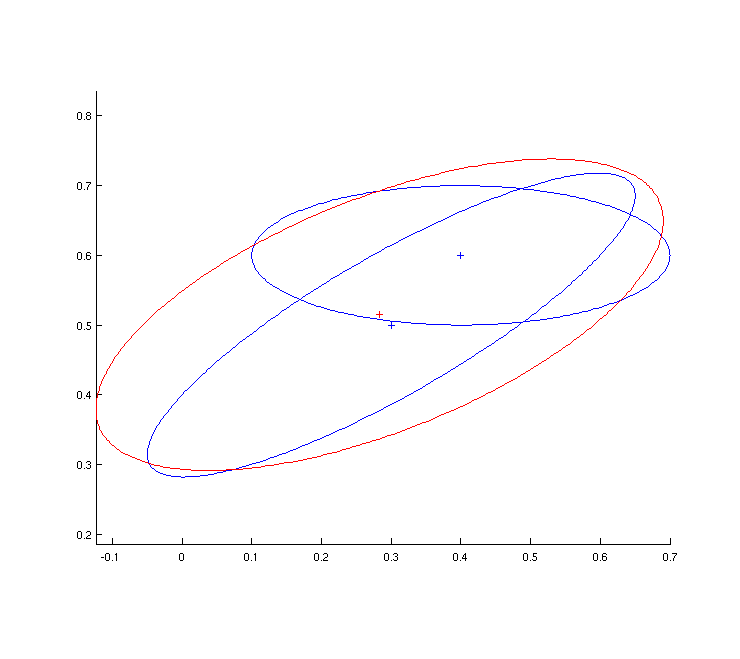
\includegraphics[width=0.6\textwidth]{figures/cu2d.png}
    \caption{\it 1-$\sigma$ contour plots of two 2D input estimates (blue) together with the CU result (red).}
    \label{fig:cu2d}
\end{figure}
\begin{align}
    \m{U}   &\geq   \m{M}_1 + (\v{u}-\v{m}_1)(\v{u}-\v{m}_1)^T\nonumber\\
    \m{U}   &\geq   \m{M}_2 + (\v{u}-\v{m}_2)(\v{u}-\v{m}_2)^T\nonumber\\
    ~       &\qquad\vdots\nonumber\\
    \m{U}   &\geq   \m{M}_n + (\v{u}-\v{m}_n)(\v{u}-\v{m}_n)^T,\label{eqn:cu}
\end{align}
for inputs $1$ to $n$. The goal of this operation is to find the location of the mean vector $\v{u}$ having the smallest
covariance $\m{U}$ that is large enough to guarantee consistency with its $n$ input estimates, regardless of which of the
$n$ estimates is consistent~\cite{fusion06,uhlmann03}.

In multimodal applications, the inputs to CU are not separate estimates of the same object to be deconflicted, but
separate modes used to represent the state of a complex or compound object. Performing CU on some or all of these modes
can be used to reduce the overall information complexity by combining modes, instead of pruning ``unimportant'' modes
(which would lead to an overestimation of the importance of the remaining modes).
This is necessary when considering the fusion of a complex set $S$ with another set $T$, which yields a combined
estimate that has $O(|S|*|T|)$ modes, formed from the Cartesian product $S\times T$. When the fused estimate exceeds the
complexity of the original estimates for each fusion step, the increasing complexity will tend to exhaust available
resources~\cite{fusion06}. The CU result is a faithful representation of all the modes it has replaced~\cite{uhlmann03}.

To reiterate, CU operates correctly even if one or more of its modes are inconsistent (as long as one is consistent), at
the cost of a much larger (less certain) error covariance that the Kalman filter or CI would provide.


% MOTIVATION for GCU
\section{Motivation for Generalized Covariance Union}\label{section:motivation}

The use of Covariance Union in data fusion is intended to guarantee consistency in the presence of spurious
data. CU is only useful if it will produce a result that is consistent with all of its inputs. However, a common
scenario arises in which CU will generate a result that is consistent with only one of its inputs (and inconsistent with
some or all of the others).

Consider the set of measurements $(\v{m}_1,\m{M}_1),(\v{m}_2,\m{M}_2),(\v{m}_3,\m{M}_3)$, which must be combined using
CU. The union may be computed in two ways:
\begin{enumerate}
\item {\em CU is applied to all three estimates simultaneously.}\\
    $(\v{u},\m{U})=\CU\left((\v{m}_1,\m{M}_1),(\v{m}_2,\m{M}_2),(\v{m}_3,\v{M}_3)\right)$
\item {\em CU is applied in a pair-wise fashion.}\\
    $(\v{u}',\m{U}')=\CU\left((\v{m}_1,\m{M}_1),(\v{m}_2,\m{M}_2)\right),$\\
    $(\v{u},\m{U})=\CU\left((\v{m}_3,\m{M}_3),(\v{u}',\m{U}')\right)$
\end{enumerate}
By its definition, given in equation \ref{eqn:cu}, the CU result is guaranteed to be consistent with its inputs. In the
first case, this means $(\v{u},\m{U})$ is consistent with $(\v{m}_1,\m{M}_1)$, $(\v{m}_2,\m{M}_2)$, and
$(\v{m}_3,\m{M}_3)$.  In the second case, however, all that is known for certain is that $(\v{u},\m{U})$ is consistent
with $(\v{m}_3,\m{M}_3)$ and $(\v{u}',\m{U}')$, and separately that $(\v{u}',\m{U}')$ is consistent with
$(\v{m}_1,\m{M}_1)$ and $(\v{m}_2,\m{M}_2)$. 
\begin{figure}[tbp]
    \centering
        \subfloat[First, the intermediate pairwise result is calculated.]{\label{fig:gcu-i1}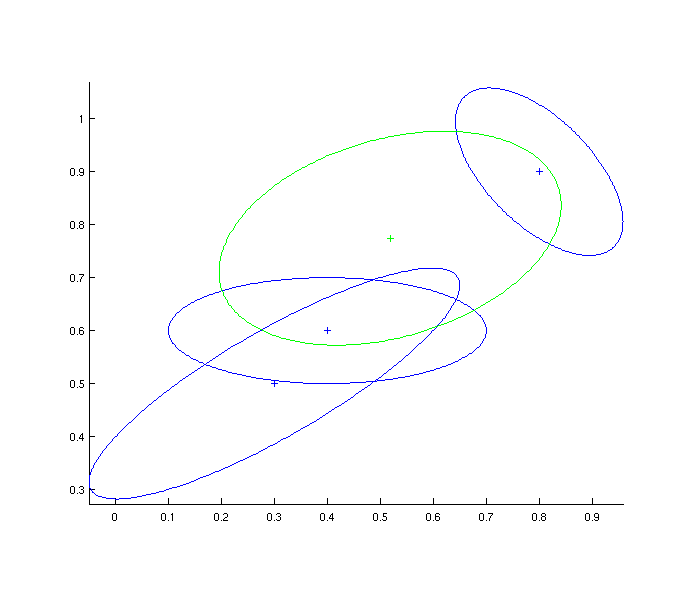
\includegraphics[width=0.4\textwidth]{figures/cu2d-i1.png}}
        \subfloat[Then, that intermediate result is used as input for the final result.]{\label{fig:gcu-iall}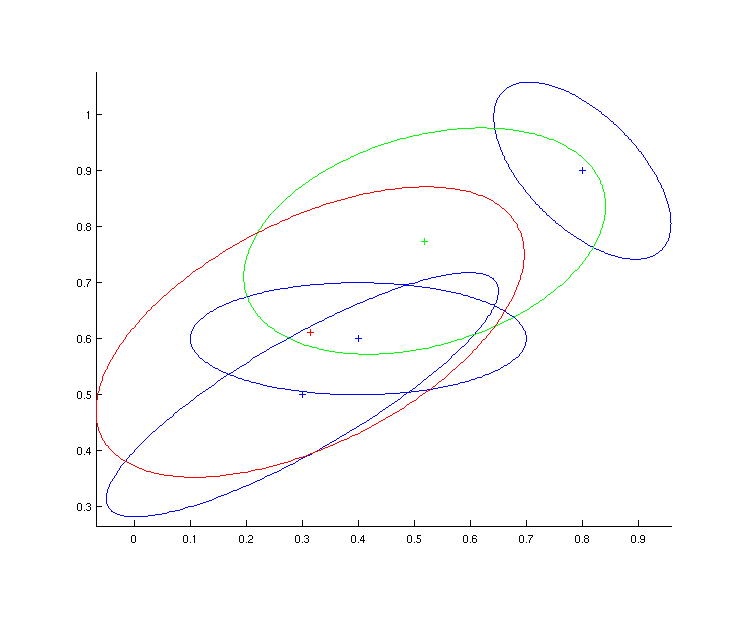
\includegraphics[width=0.4\textwidth]{figures/cu2d-iall.png}}
    \caption{\it 1-$\sigma$ contour plots of three 2D inputs (blue) together with the intermediate (pairwise) Optimal CU result
        (green) and the final (pairwise) CU result (red). Note that although the intermediate result is consistent with
        its two inputs, one of the original (blue) inputs is a clear outlier with the final (red) result.}
    \label{fig:cu2d-i}
\end{figure}

The nature of CU is to consider only the current state of the problem, i.e. its immediate inputs, and it functions with
no knowledge of any previous states. Consider an application which gathers a set of $n$ measurements at each discrete
time step, and may perform CU on some or all of those measurements for later use. If at time step $k$ CU replaces a
given estimate $(\v{m}_{i|k},\m{M}_{i|k})$ with a consistent union $(\v{u}_{k},\m{U}_{k})$, it does so by shifting the
mean from $\v{m}_{i|k}$ to $\v{u}_{k}$, and enlarging the covariance by at least the outer product of
$(\v{u}_{k}-\v{m}_{i|k})$ \cite{uhlmann03}. But if the estimate $(\v{u}_{k},\m{U}_{k})$ is used at time step $k+1$ as an
input to another CU operation, $\CU_{k+1}$ will have no knowledge of the mean shift that occurred during $\CU_{k}$. Since
CU finds the optimal, i.e. the tightest, covariance possible for all the inputs, any mean shifting that occurred during
prior time steps may cause this optimal covariance to be inconsistent for the inputs to those prior time steps
\cite{fusion06}.


% GCU
\section{Formulation of Generalized Covariance Union}\label{section:gcu}
In order to address the problems with Optimal CU as defined in section \ref{section:cu}, with regard to inconsistencies
that arise from a pair-wise or time-sequence application as described in section \ref{section:motivation}, it is
necessary to use Generalized CU. The generalized form of CU includes an additional parameter $\alpha_i$ per estimate in
the constraint equations. As with Optimal CU, the goal is to minimize some measure of $\m{U}$, e.g. the determinant. The
constraints are
\begin{figure}[tbp]
    \centering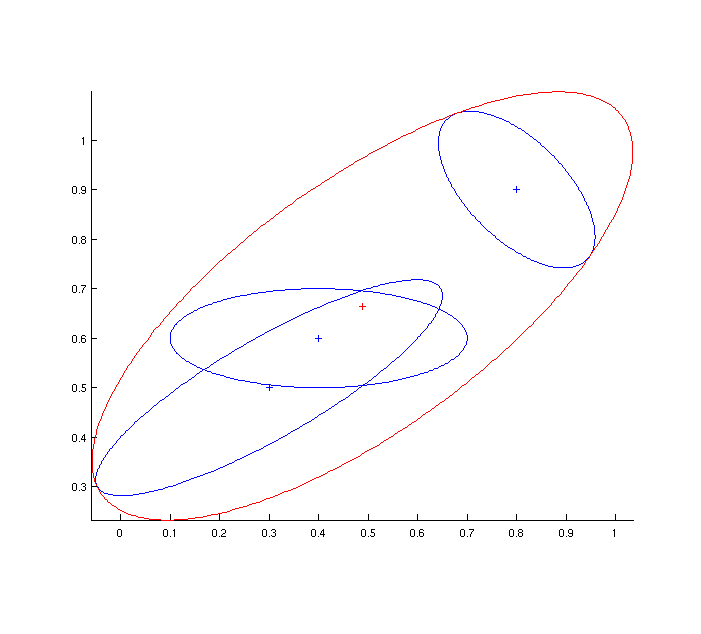
\includegraphics[width=0.6\textwidth]{figures/cu2d-gen-batch.png}
    \caption{\it 1-$\sigma$ contour plots of three 2D inputs (blue) together with the batch Generalized CU result (red).
        This is the first time that these 1-$\sigma$ plots appear to exhibit a minimally enclosing behavior.}
    \label{fig:cu2d-gen-batch}
\end{figure}
\begin{align}
    \m{U}   &\geq    \frac{\m{M}_1}{\alpha_1} + \frac{(\v{u}-\v{m}_1)(\v{u}-\v{m}_1)^T}{1-\alpha_1}\nonumber\\
    \m{U}   &\geq    \frac{\m{M}_2}{\alpha_2} + \frac{(\v{u}-\v{m}_2)(\v{u}-\v{m}_2)^T}{1-\alpha_2}\nonumber\\
    ~       &\qquad\vdots\nonumber\\
    \m{U}   &\geq    \frac{\m{M}_n}{\alpha_n} + \frac{(\v{u}-\v{m}_n)(\v{u}-\v{m}_n)^T}{1-\alpha_n},\label{eqn:gcu}
\end{align}
where $\alpha_1\dots\alpha_n$ are in the range $(0,1)$ \cite{fusion06}. Each $\alpha_i$ is equivalent to the $\omega$
parameter in equation \ref{eqn:cijointcov}~\cite{uhlmann03}, in this context used to prevent either a single covariance
$\m{M}_i$ or a single mean shift term $(\v{u}-\v{m}_i)$ from dominating the CU calculation. The $\alpha_i$ parameters
are optimized as part of this calculation to generate the tightest union possible~\cite{fusion06}. The result is
sub-optimal, but it is necessary to use this form of CU if it is used as part of a pair-wise or time-sequence
application as described above.  Generalized CU guarantees consistency regardless of how many times its result is
re-used in future CU operations.
\begin{figure}[tbp]
    \centering
        \subfloat[First, the intermediate pairwise result is calculated.]{\label{fig:gcu-s1}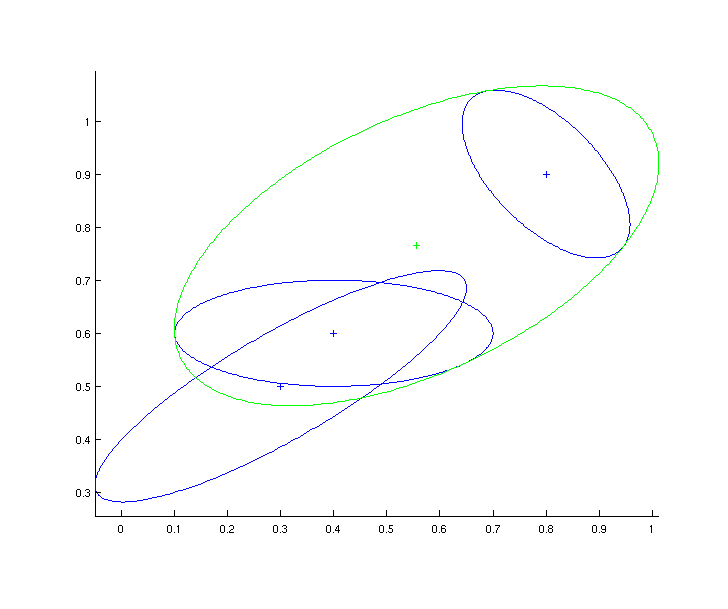
\includegraphics[width=0.4\textwidth]{figures/cu2d-gen-s1.png}}
        \subfloat[Then, that intermediate result is used as input for the final result.]{\label{fig:gcu-sall}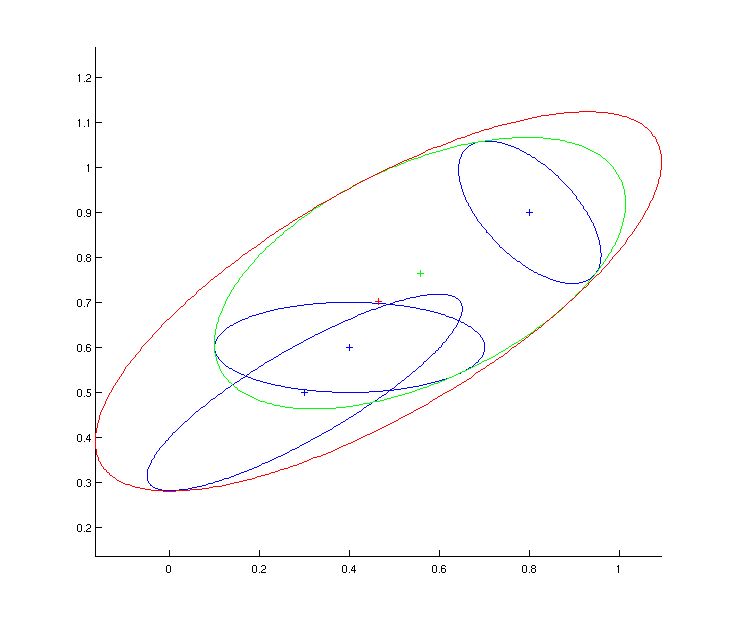
\includegraphics[width=0.4\textwidth]{figures/cu2d-gen-sall.png}}
    \caption{\it 1-$\sigma$ contour plots of three 2D inputs (blue) together with the intermediate (pairwise) Generalized CU result
        (green) and the final (pairwise) GCU result (red). Note that the final (red) result is consistent with all of
        its inputs, including all the original (blue) inputs, even those that were not used as direct inputs.}
    \label{fig:cu2d-gen-s}
\end{figure}
Figure \ref{fig:cu2d-gen-batch} shows GCU applied as a single batch operation, and figure \ref{fig:cu2d-gen-s} shows GCU
applied pairwise to the same three input estimates. The pairwise application of GCU is shown for completeness, but the
batch application is of main interest. It is this batch GCU operation, specifically its 1-$\sigma$ contour ellipsoid,
which will be compared to the MEEE problem.





\typeout{}
\chapter{Minimal Enclosing Ellipsoid of Ellipsoids}\label{chapter:meee}

\section{Uses of MEEE}

\PARstart{T}{he idea} of approximating complicated objects using simpler ones is widely used in computational geometry
and computer graphics. A common approach is to replace a complicated object by a simpler model covering it, such as a
minimum volume box or a sphere. More recently, ellipsoidal models have been proposed in the literature as they usually
provide better approximations than bounding boxes or spheres~\cite{yildirim06,sturm03,shiang00,ju01}. The use of simpler
objects inevitably leads to faster processing times for more responsive applications, ideally with minimal---though not
insignificant---loss of detail resolution. Recently new algorithms have been developed for the calculation of a minimal
enclosing ellipsoid; specifically, such an ellipsoid bounding the convex hull of a set of ellipsoids, also known as a
L\"owner ellipsoid, or L\"owner-John ellipsoid~\cite{yildirim06}.


% MAXDET 
\section{Solving with MAXDET}

The maxdet-problem is a convex optimization problem, minimizing the objective function
\begin{equation}\label{eqn:maxdetobj}
    c^T\v{x} + \log \det G(\v{x})^{-1}
\end{equation}
subject to
\begin{align}
     G(\v{x}) &>     0,\qquad\text{and}\nonumber\\
     F(\v{x}) &\geq  0,\label{eqn:maxdetcons}
\end{align}
where the optimization variable is the vector $\v{x}\in\Re^m$. The Functions 
$G:\Re^m\rightarrow\Re^{\left|\v{x}\right|}$ and $F:\Re^m\rightarrow\Re^{n\times n}$ are affine:
\begin{align}
    G(\v{x}) &= G_0 + \v{x}_1G_1 + \dots + \v{x}_mG_m\nonumber\\
    F(\v{x}) &= F_0 + \v{x}_1F_1 + \dots + \v{x}_mF_m\label{eqn:maxdet},
\end{align} 
where $G_i=G_i^T$ and $F_i=F_i^T$. The objective function is convex on $\{x|G(x)>0\}$ and the constraint set is
convex~\cite{vandenberghe96}.

A wide class of computational geometry problems can be formulated at maxdet-problems. The formulation of interest is
that of a minimal volume ellipsoid $\varepsilon_0$ containing $n$ given ellipsoids $\varepsilon_1\dots\varepsilon_n$. The
given ellipsoids are described as sublevel sets of convex quadratic functions:~\cite{vandenberghe96,boyd04}
\begin{equation}\label{eqn:ellipse}
    \varepsilon_i = \{ x | x^TA_ix + 2b_i^Tx + c_i \leq 0 \},\qquad i=0,\dots,n.
\end{equation}
The solution can be found by, in the variables $A_0 = A_0^T$, $b_0$, and
$n$ scalar variables $\tau_i$, minimizing:~\cite{vandenberghe96}
\begin{equation}\label{eqn:maxdetfun}
    \log\det A_0^{-1}
\end{equation}
subject to
\begin{equation}\label{eqn:maxdetconstraints}
    \begin{array}{l}
    A_0 = A_0^T > 0 ,\\
    \tau_1 \geq 0,\dots,\tau_n\geq 0 ,\qquad\text{and}\\
    \left[ \begin{array}{ccc}
        A_0   & b_0 &  0     \\
        b_0^T & -1  & b_0^T  \\
        0     & b_0 & -A_0
    \end{array} \right]
    -\tau_i
    \left[ \begin{array}{ccc}
        A_i   & b_i & 0 \\
        b_i^T & c_i & 0 \\
        0     &   0 & 0 
    \end{array} \right]
    \leq 0,\qquad i=1,\dots,n.
    \end{array}
\end{equation}
Here, $c_0$ is given by~\cite{boyd94}
\begin{equation}
    c_0=b_0^TA_0^{-1}b_0-1\\
\end{equation}
and the final ellipsoid is
\begin{equation}
    \varepsilon_0=\{x|x^TA_0x+2b_0^Tx+c_0\leq 0\},
\end{equation}
which defines the ellipsoid of least volume containing $\varepsilon_1,\dots,\varepsilon_n$. The formulation for the MEEE
constraints given in equation \ref{eqn:maxdetconstraints} as a maxdet-problem, as in equation \ref{eqn:maxdet}, 
is~\cite{vandenberghe96}.
\begin{align}
    G(\v{x}) &= I_{n\times n}\nonumber\\
    F(\v{x}) &= \left[\begin{array}{cccc}
        A_0 &   &  &  \\
            & \left[ \begin{array}{ccc}
                \tau_i A_i - A_0   & \tau_i b_i - b_0 &  0     \\
                \tau_i b_i^T - b_0^T & \tau_i c_i -1  & -b_0^T  \\
                0     & -b_0 & A_0
                \end{array}\right]  &  &  \\
            &   & \ddots & \\
            &   &  & 
                \left[ \begin{array}{ccc}
                \tau_1 &  &  \\
                       & \ddots & \\
                       &       & \tau_n
            \end{array}\right]
    \end{array}\right]
\end{align}
The variables $A_0$ and $b_0$, and $\tau_1\dots \tau_n$, are solved in-place during the minimization process.
\begin{figure}[tbp]
    \centering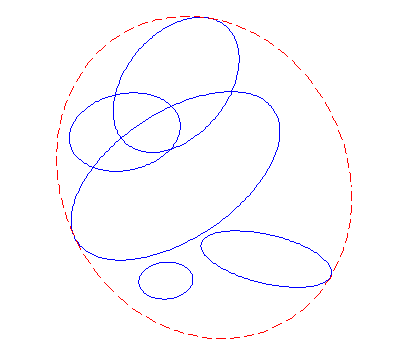
\includegraphics[width=0.6\textwidth]{figures/ellipse01.png}
    \caption{\it An example of a minimally enclosing L\"owner 2D ellipsoid containing five ellipsoids,
        from~\cite{boyd04}. Comparing this plot with figure \ref{fig:cu2d-gen-batch} will illustrate the superficial
        similarities between GCU and MEEE. }
    \label{fig:ellipse}
\end{figure}

Other convex optimization tools may be easily used with the objective function and constraints given in equations
\ref{eqn:maxdetfun} and \ref{eqn:maxdetconstraints} as well~\cite{boyd04}.


% CONTAINMENT
\section{Testing for Ellipsoid Containment}\label{section:containment}

In the development of any algorithm which finds a minimally enclosing object, it is necessary to also develop a test to
compare this theoretically enclosing result with its enclosed set. For the MEEE problem, the goal is to test whether one
ellipsoid properly contains another, i.e. the properly contained ellipsoid does not have any points which fall outside
the bounding perimeter of the containing ellipsoid~\cite{yildirim06}.

This analysis follows the test for ellipse intersection presented in~\cite{eberly00}. Consider an $n$--dimensional
ellipsoid $\varepsilon_0$ given by the curve,
\begin{equation}
    Q_0 = x^TA_0x + 2b_0^Tx + c_0,
\end{equation}
which should contain the $n$--dimensional ellipsoid $\varepsilon_1$ given by the curve,
\begin{equation}
    Q_1 = x^TA_1x + 2b_1^Tx + c_1.
\end{equation}
All level curves defined by $Q_0(x)=\lambda$ are ellipsoids, except for the minimum negative value of $\lambda$ for
which the equation defined a single point, the center of every level curve ellipsoid. The ellipsoid defined by
$Q_1(x)=0$ generally intersects many level curves of $Q_0$. By finding the minimum level value $\lambda_{min}$ and the
maximum level value $\lambda_{max}$ of $Q_0$ attained by any $x$ on the curve $Q_1$, it is possible to determine the
spatial relationship between $\varepsilon_0$ and $\varepsilon_1$. If $\lambda_{max}\leq 0$, then only a level curve
$Q_0(x)\leq 0$ will intersect $Q_1(x)=0$, and $\varepsilon_0$ must properly contain $\varepsilon_1$.

This can be formulated as a constrained minimization that can be solved by the method of Lagrange multipliers: Minimize
$Q_0(x)$ subject to the constraint that $Q_1(x)=0$. Define $F(x,t)=Q_0(x)+tQ_1(x)$. Differentiating yields $\nabla
F=\nabla Q_0+t\nabla Q_1$, where the gradient indicated derivative in $x$. Since $\partial{F}/\partial{t}=Q_1$, setting the
$t$-derivative equal to zero reproduces the constraint $Q_1=0$. Setting the $x$-derivative equal to zero yields $\nabla
Q_0+t\nabla Q_1=0$ for some $t$. Geometrically, this means the gradients are parallel.

Note that $\nabla Q_i=2A_ix+2b_i$, so
\begin{equation}
    0 = \nabla Q_0 + t\nabla Q_1 = 2(A_0+tA_1)x+2(b_0+tb_1).
\end{equation}
Solving for $x$ yields
\begin{equation}\label{eqn:solvex}
    x = -(A_0+tA_1)^{-1}(b_0+tb_1)=\frac{1}{\delta(t)}Y(t),
\end{equation}
where $\delta(t)$ is the determinant of $(A_0+tA_1)$, a polynomial in $t$ of degree $n$, and $Y(t)$ has components in
$t$ of degree $n$ as well. Replacing this in $Q_1(x)=0$ yields
\begin{equation}\label{eqn:poly}
    P(t) = Y(t)^TA_1Y(t)+\delta(t)b_1^TY(t)+\delta(t)^2c_1=0,
\end{equation}
a degree $2n$ polynomial in $t$. The roots of $P(t)$ in equation \ref{eqn:poly} can be applied to equation
\ref{eqn:solvex} to find the critical values for $x$ of $Q_1$. The minimum and maximum values of the evaluation of
$Q_0(x)$ at the roots of $P(t)$ are respectively $\lambda_{min}$ and $\lambda_{max}$, the minimum and maximum level
curves which intersect $Q_1$. 

As stated previously, if $\lambda_{max}\leq 0$, then $\varepsilon_0$ properly contains $\varepsilon_1$.


% TRANSFORM
\section{Relating to Generalized Covariance Union}

Before any MEEE results can be compared to GCU, it is necessary to define a set of transforms between the ellipsoid and
statistical measurement domains.  Since this thesis interprets all estimates (means and covariances) as unweighted
Gaussian PDFs, i.e.
\begin{equation}
    (\v{m}_i,\m{M}_i) := \gaussN{\v{m}_i,\m{M}_i},
\end{equation}
each estimate is uniquely transformable to and from the ellipsoid domain, given in equation \ref{eqn:ellipse},
by representing each as only the 1-$\sigma$ contour ellipsoid on its Gaussian surface. The
forward transformation into ellipse notation is~\cite{boyd04}
\begin{align}
\label{eqn:cu2e}
\mathbb{T}(\v{m}_i,\m{M}_i) &:= \left\{
    \begin{aligned}
        A_i &= \m{M}_i^{-1}\\
        b_i &= -\m{M}_i^{-1}\v{m}_i\\
        c_i &= \v{m}_i^T\m{M}_i^{-1}\v{m}_i-1,
    \end{aligned}
    \right.
\intertext{and the backward transformation is}
\label{eqn:e2cu}
\mathbb{T}^{-1}(A_i,b_i,c_i) &:= \left\{
    \begin{aligned}
        \m{M}_i &= A_i^{-1}\\
        \m{m}_i &= -A_i^{-1}b_i.
    \end{aligned}
    \right.
\end{align}
The ellipsoid described by $(A_i,b_i,c_i)$ is centered at $\v{m}_i$, with a radial distance of $\m{M}_i^{\frac{1}{2}}$.
By interpreting a given Gaussian PDF as an ellipsoid, or a given ellipsoid as the 1-$\sigma$ contour which defines a
Gaussian PDF, it is possible to directly compare the results of GCU and MEEE.









\typeout{}
\chapter{Analysis}\label{chapter:analysis}

\section{Explanation of $\mathbf{\alpha}$--Parametrized Behavior}\label{section:explanation}

\PARstart{I}{ncluding} the $\alpha_i$ parameter in the Generalized CU constraints, given in equation \ref{eqn:gcu},
creates an asymptotic scale on which the terms $\m{M}_i$ and $(\v{u}-\v{m}_i)$ are balanced. At the two extremes are the
following cases:
\begin{enumerate}
\item If $\m{M}_i$ is a zero matrix, $\alpha_i$ is allowed to approach 0 as well, and the constraint reduces to
$\m{U}\geq (\v{u}-\v{m}_i)(\v{u}-\v{m}_i)^T$, and
\item If $\v{u}$ and $\v{m}_i$ are coincident, $\alpha_i$ is allowed to approach 1, and the constraint reduces to
$\m{U}\geq \m{M}_i$.
\end{enumerate}
For the general case, in which both terms are nonzero, the actual value of $\alpha_i$ will be bounded somewhere between
0 and 1. It is not important to know this actual value, since it is determined by the optimization process in
conjunction with the other $n-1$ estimates.

With this knowledge, it is possible to logically reduce the question of whether Generalized CU and MEEE are equivalent.
First, since it is necessary to satisfy all $n$ constraints in equation \ref{eqn:gcu}, a minimal L\"owner
ellipsoid $\varepsilon_0$ for $(\v{u},\m{U})$ will be one that completely contains the ellipsoid $\varepsilon_i$ for
each $(\v{m}_i,\m{M}_i)$ in $i=1\dots n$~\cite{yildirim06}. Second, if the ellipsoid $\tau_i$ for
$(\v{u},\frac{\m{M}_i}{\alpha_i}+\frac{(\v{u}-\v{m}_i)(\v{u}-\v{m}_i)^T}{1-\alpha_i})$ completely contains
$\varepsilon_i$, it follows that $\varepsilon_0$ will completely contain $\varepsilon_i$ as well, since $\tau_i$ and
$\varepsilon_0$ are both centered at $\v{u}$ and $\varepsilon_0$ is at least as large as $\tau_i$. Therefore, if
$\tau_i$ can be shown to completely enclose $\varepsilon_i$ for all values of $\alpha_i\in (0,1)$, for
all $i=1\dots n$, then $\varepsilon_0$ is a L\"owner ellipsoid, and Generalized CU and MEEE are in fact equivalent.

Formally, $\varepsilon_i$ and $\tau_i$ are the 1-$\sigma$ ellipsoids transformed by equation \ref{eqn:cu2e}; of
\begin{align}
    \displaystyle
    \varepsilon_i    &= \mathbb{T}\left(\v{m}_i,\m{M}_i\right)\label{eqn:coveps}\\
    \tau_i(\alpha_i) &=
\mathbb{T}\left(\v{u},\frac{\m{M}_i}{\alpha_i}+\frac{(\v{u}-\v{m}_i)(\v{u}-\v{m}_i)^T}{1-\alpha_i}\right)\label{eqn:covtau}
\end{align}
The containing ellipsoid $\tau_i$ varies with $\alpha_i$, with all other terms constant. An analysis of this behavior
follows.


% 1D
\section{Describing the Behavior in One Dimension}

Since the 1-$\sigma$ ellipsoid of a Gaussian curve in one variable is a line, the mathematics are extremely simple; it
becomes extremely easy to visualize and plot the data, and to check the results by hand. Notationally,
$(\v{m}_i,\m{M}_i)$ is just $(\mu_i,\sigma_i^2)$, and the PDF of the estimate is given by the unweighted Gaussian
function
\begin{equation}\label{eqn:gauss1d}
    \varphi_{\mu_i,\sigma_i^2}(x)=e^\frac{-(\mu_i-x)^2}{2\sigma_i^2}, \end{equation}
and the 1-$\sigma$ ellipsoid is the band between $\mu_i-1\sigma_i$ and $\mu_i+1\sigma_i$. The $y$ value of the
1-$\sigma$ line is $\varphi_{\mu_i,\sigma_i^2}(x=\mu_i\pm\sigma_i)=e^{-\frac{1}{2}}\approx0.6065$.

% EXAMPLE 1D CU
\begin{example}[Generalized CU in One Dimension]\label{ex:gcu1d}

Consider a set of four estimates $(\mu_i,\sigma_i^2)$, given by
\begin{figure}[tbp]
    \centering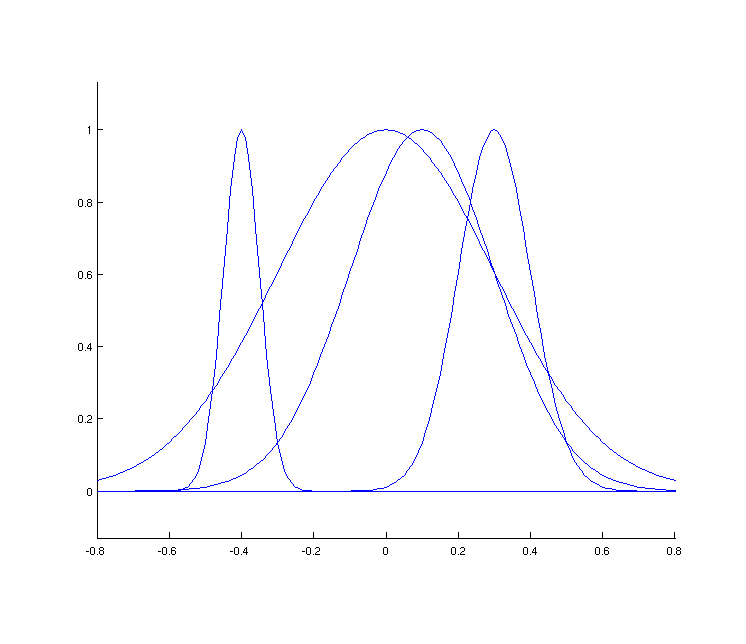
\includegraphics[width=0.6\textwidth]{figures/est1d-4.png}
    \caption{\it 1D Gaussian curves for four estimate means and covariances, for example \ref{ex:gcu1d}.}
    \label{fig:est1d-4}
\end{figure}
\begin{align}
    (\mu_1,\sigma_1^2) &= (0.3000,0.1000^2)\\\nonumber
    (\mu_2,\sigma_2^2) &= (0.1000,0.2000^2)\\\nonumber
    (\mu_3,\sigma_3^2) &= (0.0000,0.3000^2)\\\nonumber
    (\mu_4,\sigma_4^2) &= (-0.4000,0.0500^2),\label{ex:est1d-4}
\end{align}
shown in figure \ref{fig:est1d-4}. Applying batch Generalized CU to these inputs,
\begin{equation}
    (\mu_u,\sigma_u^2) = \GCU\left((\mu_1,\sigma_1^2),(\mu_2,\sigma_2^2),(\mu_3,\sigma_3^2),(\mu_4,\sigma_4^2)\right)
\end{equation}
yields the values
\begin{figure}[tbp]
    \centering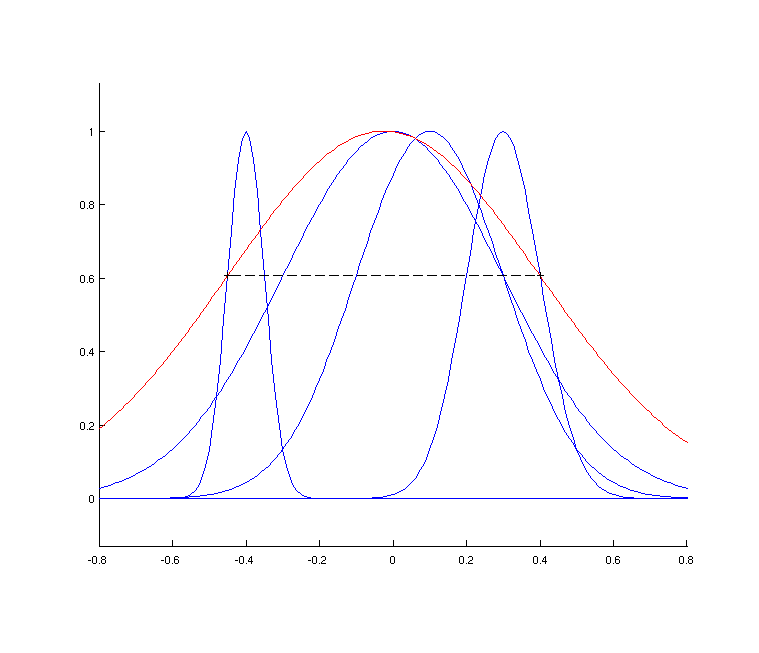
\includegraphics[width=0.6\textwidth]{figures/cu1d.png}
    \caption{\it 1D Gaussian curves for four inputs (blue), together with the batch Generalized CU result (red) and
            its 1-$\sigma$ ellipsoid (dashed), for example \ref{ex:gcu1d}.}
    \label{fig:cu1d}
\end{figure}
\begin{equation}
    (\mu_u,\sigma_u^2) = (-0.0250,0.4250^2).
\end{equation}
Figure \ref{fig:cu1d} shows the inputs plotted with the Gaussian curve for $(\mu_u,\sigma_u^2)$. The 1-$\sigma$ line,
from $x=\mu_u-\sigma_u$ to $x=\mu_u+\sigma_u$, at $y=e^{-\frac{1}{2}}$, corresponds to the outermost intersection points
between the inputs and the CU result curves. The boundary points for each 1-$\sigma$ ellipsoid are $x=\mu_i\pm\sigma_i$:
\begin{align}
    \mu_1-\sigma_1 &= 0.2000 & \mu_1+\sigma_1 &= 0.4000\nonumber\\
    \mu_2-\sigma_2 &= -0.1000 & \mu_2+\sigma_2 &= 0.3000\nonumber\\
    \mu_3-\sigma_3 &= -0.3000 & \mu_3+\sigma_3 &= 0.3000\nonumber\\
    \mu_4-\sigma_4 &= -0.4500 & \mu_4+\sigma_4 &= -0.3500\\
\intertext{Of these points, $\mu_4-\sigma_4$ and $\mu_1+\sigma_1$ exactly equal the 1-$\sigma$ points on the CU curve,}
    \mu_u-\sigma_u &= -0.4500 & \mu_u+\sigma_u &= 0.4000,
\end{align}
and the remaining points are all within the range $(-0.4500,0.4000)$.

Following the logic outlined in section \ref{section:explanation}, it is
necessary to consider the ellipsoid $\varepsilon_1$ from equation \ref{eqn:coveps} and $\tau_1(\alpha_1)$ from equation
\ref{eqn:covtau}:
\begin{align}
    \varepsilon_1 &= \mathbb{T}\left(\mu_1,\sigma_1^2\right) = \mathbb{T}\left(0.3000,0.0100\right)\\
    \tau_1(\alpha_1) &= \mathbb{T}\left(\mu_u,\frac{\sigma_1^2}{\alpha_1}+\frac{(\mu_u-\mu_1)^2}{1-\alpha_1}\right)
        = \mathbb{T}\left(-0.0250,\frac{0.0100}{\alpha_1}+\frac{0.1056}{1-\alpha_1}\right).
\end{align}
From equation \ref{eqn:cu2e}, the transformation into ellipsoid space is:
\begin{align}
    \varepsilon_1 &= \left\{
        \begin{aligned}
            A_{\varepsilon,1} &= 100\\
            b_{\varepsilon,1} &= -30\\
            c_{\varepsilon,1} &= 8
        \end{aligned}\right.,\\\nonumber
    \tau_1(\alpha_1) &= \left\{
        \begin{aligned}
            A_{\tau,1} &= \frac{\begin{smallmatrix}1\end{smallmatrix}}{\frac{0.0100}{\alpha_1}+\frac{0.1056}{1-\alpha_1}} \\
            b_{\tau,1} &= \frac{\begin{smallmatrix}0.0250\end{smallmatrix}}{\frac{0.0100}{\alpha_1}+\frac{0.1056}{1-\alpha_1}} \\
            c_{\tau,1} &= \frac{\begin{smallmatrix}0.0062\end{smallmatrix}}{\frac{0.0100}{\alpha_1}+\frac{0.1056}{1-\alpha_1}} -1 \\
        \end{aligned}\right.
\end{align}
Equation \ref{eqn:ellipse} (repeated here)
\begin{equation}
    \varepsilon_i = \{ x | x^TA_ix + 2b_i^Tx + c_i \leq 0 \}\nonumber
\end{equation}
gives the quadratic formulation for an $n$-dimensional ellipsoid. In one dimension, $\varepsilon_1$ can be written as
\begin{equation}
    \varepsilon_1 = 100x^2-60x+8 \leq 0,
\end{equation}
and solving for the roots gives
\begin{equation}
    x = 0.2, \qquad x = 0.4,
\end{equation}
which are exactly equal to $\mu_1\pm\sigma_1$. For $\tau_1(\alpha_1)$ to completely contain $\varepsilon_1$, its roots
must bound the roots of $\varepsilon_1$ for all values of $\alpha_1\in(0,1)$.
\begin{figure}[tbp]
    \centering
        \subfloat[$\alpha_1$=0.05]{\label{fig:alpha1d05}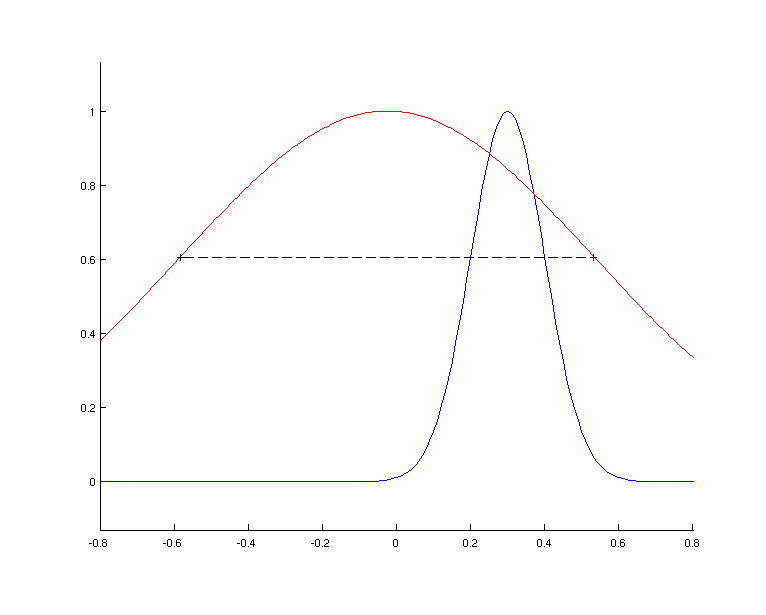
\includegraphics[width=0.4\textwidth]{figures/alpha1d-05.png}}
        \subfloat[$\alpha_1$=0.25]{\label{fig:alpha1d25}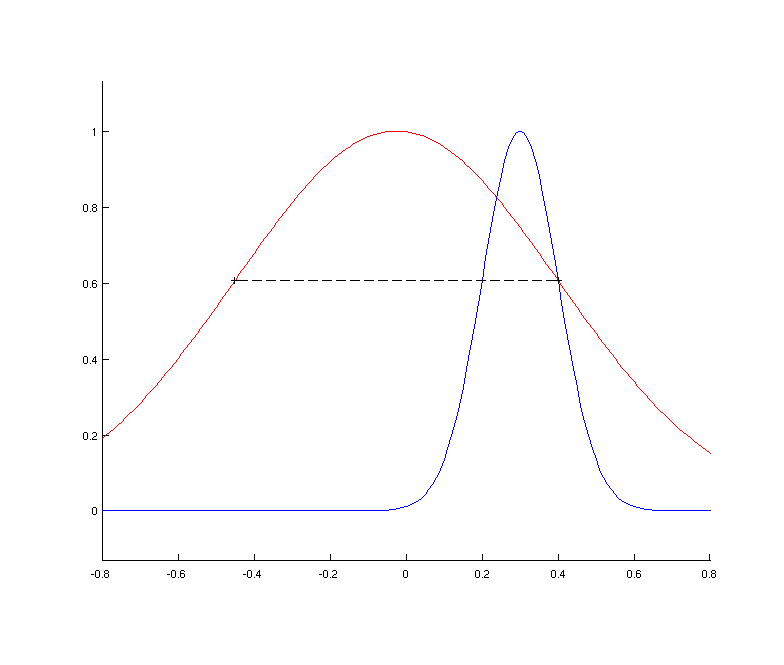
\includegraphics[width=0.4\textwidth]{figures/alpha1d-25.png}}
        \subfloat[$\alpha_1$=0.50]{\label{fig:alpha1d50}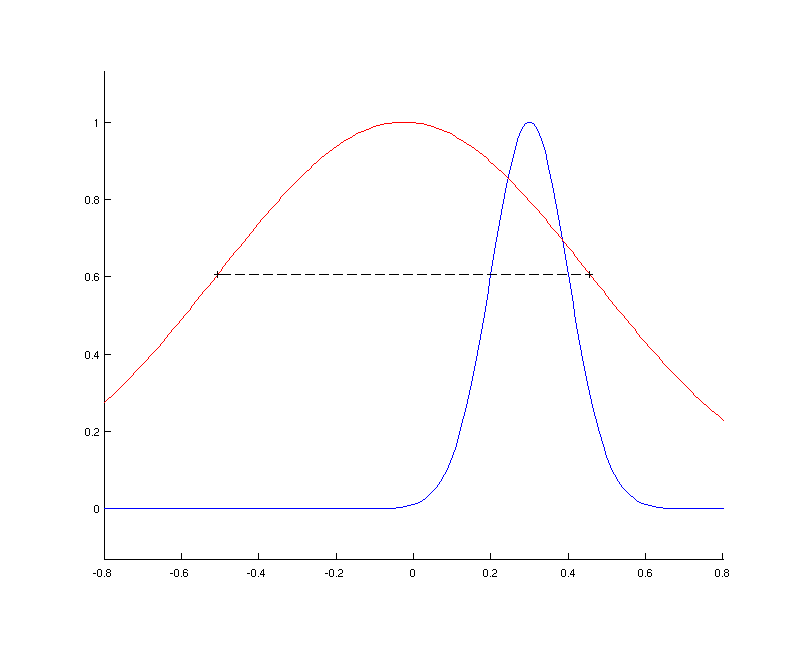
\includegraphics[width=0.4\textwidth]{figures/alpha1d-50.png}}
        \subfloat[$\alpha_1$=0.75]{\label{fig:alpha1d75}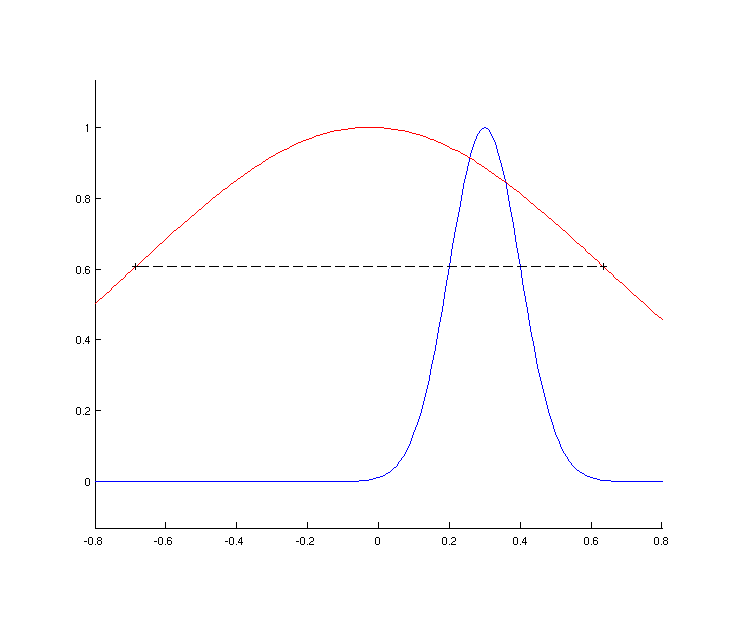
\includegraphics[width=0.4\textwidth]{figures/alpha1d-75.png}}
        \subfloat[$\alpha_1$=0.95]{\label{fig:alpha1d95}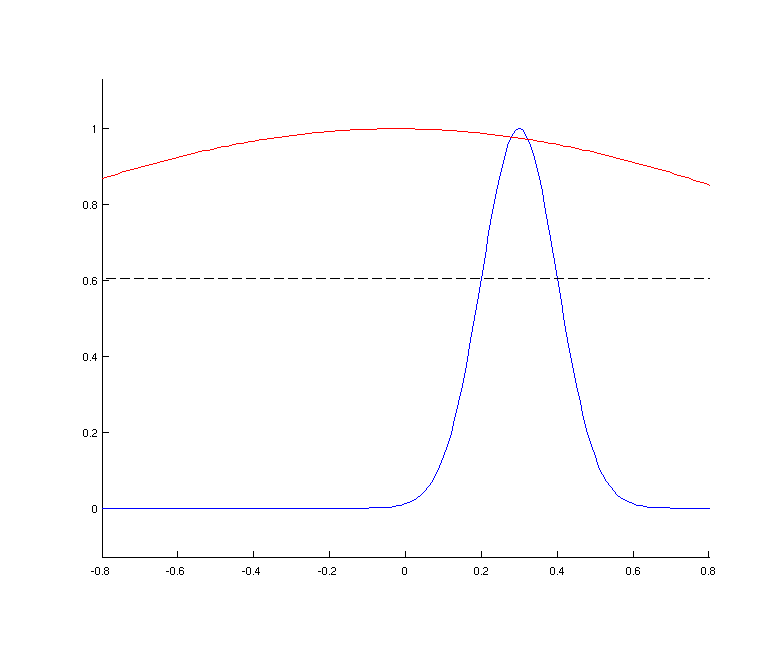
\includegraphics[width=0.4\textwidth]{figures/alpha1d-95.png}}
    \caption{\it 1D Gaussian curves for estimate $(\v{m}_1,\m{M}_1)$ and the intermediate error covariance (red), and
            its 1D 1-$\sigma$ ellipsoid (dashed), for example \ref{ex:gcu1d}.}
    \label{fig:alpha1d}
\end{figure}
By choosing a value for $\alpha_1$, it is possible to numerically determine the intermediate error covariance
$\left(\mu_u,\frac{\sigma_1^2}{\alpha_1}+\frac{(\mu_u-\mu_1)^2}{1-\alpha_1}\right)$, and the 1-$\sigma$ ellipsoid
$\tau_1(\alpha_1)$ and its roots. Using the ellipsoid transformation (equation \ref{eqn:cu2e}) and quadratic ellipsoid
equation (\ref{eqn:ellipse}) as above, the roots of $\tau_1(\alpha_1)$ are:
\begin{equation}
    x = \begin{cases}
            -0.5828, 0.5328 \qquad \text{for $\alpha_1 = 0.05$}\\
            -0.4502, 0.4002 \qquad \text{for $\alpha_1 = 0.25$}\\
            -0.5059, 0.4559 \qquad \text{for $\alpha_1 = 0.50$}\\
            -0.6852, 0.6352 \qquad \text{for $\alpha_1 = 0.75$}\\
            -1.4821, 1.4321 \qquad \text{for $\alpha_1 = 0.95$}
        \end{cases}
\end{equation}
\begin{figure}[tbp]
    \centering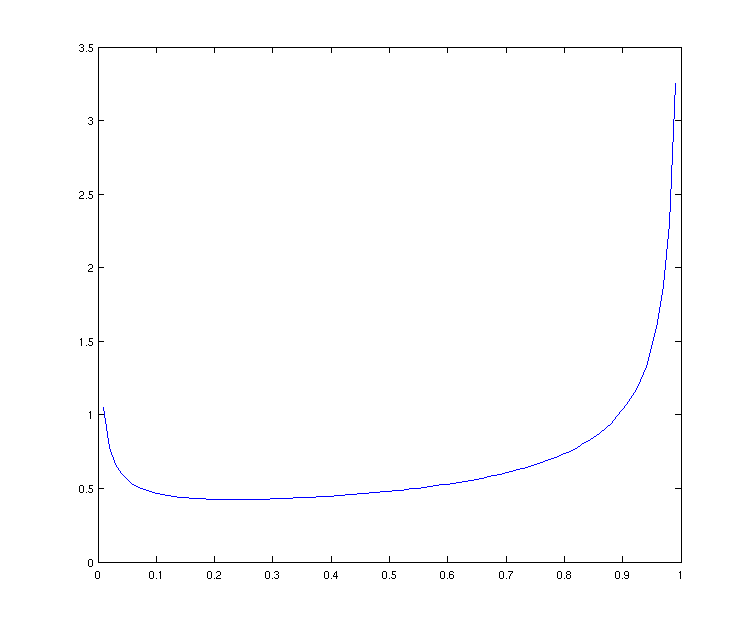
\includegraphics[width=0.6\textwidth]{figures/alpha1dcurve.png}
    \caption{\it $\alpha_1$ vs $\sigma_{intermediate,1}$ for example \ref{ex:gcu1d}.}
    \label{fig:alpha1dcurve}
\end{figure}
Since the roots of $\tau_1(\alpha_1)$ can also be written as $\mu_u\pm\sigma_{intermediate,1}$, it is also useful to
find the value of the intermediate standard deviation
\begin{equation}
    \sigma_{intermediate,1} = \sqrt{\frac{\sigma_1^2}{\alpha_1}+\frac{(\mu_u-\mu_1)^2}{1-\alpha_1}}
\end{equation}
and plot it versus $\alpha_1$, as shown in figure \ref{fig:alpha1dcurve}. The minimum value for
$\sigma_{intermediate,1}$ occurs at $\alpha_1=0.2350$, so the smallest ellipsoid $\tau_1(\alpha_1)$ is:
\begin{equation}
    \tau_1(\alpha_1=0.2350) = \left\{
        \begin{aligned}
            A_{\varepsilon,1} &= 5.5373\\
            b_{\varepsilon,1} &= 0.1384\\
            c_{\varepsilon,1} &= -0.9654
        \end{aligned}\right.
\end{equation}
The quadratic form is
\begin{equation}
    \varepsilon_1 = 5.5373x^2+2768x-0.9654 \leq 0,
\end{equation}
and solving for the roots gives
\begin{equation}
    x = -0.4499, \qquad x = 0.3999,
\end{equation}
which are within acceptable floating-point rounding error of $\mu_u\pm\sigma_{intermediate,1}$.

This procedure can be repeated for $(\mu_2,\sigma_2^2)$, $(\mu_3,\sigma_3^2)$, and $(\mu_4,\sigma_4^2)$ to confirm the
same behavior. The fact that the roots of $\varepsilon_i$ are bounded by the roots of $\tau_i(\alpha_i)$ for all
$\alpha_i\in(0,1)$ implies that $\varepsilon_0 = \mathbb{T}\left(\mu_u,\sigma_u^2\right)$ completely contains each
$\varepsilon_i$, and is therefore a minimal L\"owner ellipsoid.

\end{example}

% 2D
\section{Describing the Behavior in Two Dimensions}

In two dimensions, relative positions between estimate means become more complex, and additionally rotations must be
considered for each covariance body. Regarding notation, $\v{m}_i$ is
$\left[\begin{smallmatrix}\mu_{x,i}\\\mu_{y,i}\end{smallmatrix}\right]$ and $\m{M}_i$ is at least as large as
$\left[\begin{smallmatrix}\sigma_{x,i}\\\sigma_{y,i}\end{smallmatrix}\right]
 \left[\begin{smallmatrix}\sigma_{x,i}&\sigma_{y,i}\end{smallmatrix}\right]$, though $\sigma_{x,i}$ and $\sigma_{y,i}$
may be rotated by any arbitrary amount. The PDF of the estimate is given by the unweighted Gaussian function
\begin{equation}\label{eqn:gauss2d}
    \varphi_{(\mu_{x,i},\mu_{y,i}),(\sigma_{x,i},\sigma_{y,i})} = 
        e^{-\left(\frac{(\mu_{x,i}-x)^2}{2\sigma_{x,i}^2}\right)-\left(\frac{(\mu_{y,i}-y)^2}{2\sigma_{y,i}^2}\right)},
\end{equation}
and the 1-$\sigma$ ellipsoid is a two dimensional ellipse centered at $(\mu_{x,i},\mu_{y,i})$ with axes of length
$2\sigma_{x,i}$ and $2\sigma_{y,i}$, rotated to match $\varphi_{(\mu_{x,i},\mu_{y,i}),(\sigma_{x,i},\sigma_{y,i})}$. The
behavior of the $\alpha$--parametrized intermediate covariance is also more complex, since it is a linear combination
of both the shape of $\m{M}_i$ and the relative distance between the means $\v{m}_i$ and $\v{u}$.


% EXAMPLE 2D CU
\begin{example}[Generalized CU in Two Dimensions]\label{ex:gcu2d}

Consider as set of four estimates $(\v{m}_i,\m{M}_i)$, given by
\begin{figure}[tbp]
    \centering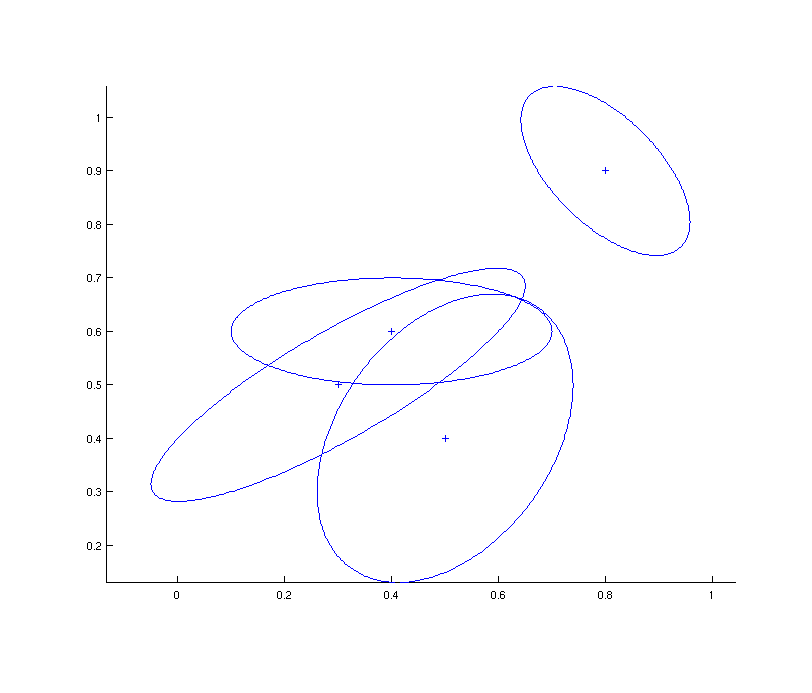
\includegraphics[width=0.6\textwidth]{figures/est2d-4.png}
    \caption{\it 1-$\sigma$ contour ellipsoids for four 2D input estimate means and covariances used in example \ref{ex:gcu2d}.}
    \label{fig:est2d-4}
\end{figure}
\begin{align}
    (\v{m}_1,\m{M}_1) &= \left(\left[
        \begin{smallmatrix}
            0.3000\\
            0.5000
        \end{smallmatrix}\right],
        \left[
        \begin{smallmatrix}
            0.1225 &  0.0650\\
            0.0650 &  0.0475
        \end{smallmatrix}\right]\right)\nonumber\\
    (\v{m}_2,\m{M}_2) &= \left(\left[
        \begin{smallmatrix}
            0.4000\\
            0.6000
        \end{smallmatrix}\right],
        \left[
        \begin{smallmatrix}
            0.0900 &  0.0000\\
            0.0000 &  0.0100
        \end{smallmatrix}\right]\right)\nonumber\\
    (\v{m}_3,\m{M}_3) &= \left(\left[
        \begin{smallmatrix}
            0.8000\\
            0.9000
        \end{smallmatrix}\right],
        \left[
        \begin{smallmatrix}
            0.0250 & -0.0150\\
           -0.0150 &  0.0250
        \end{smallmatrix}\right]\right)\nonumber\\
    (\v{m}_4,\m{M}_4) &= \left(\left[
        \begin{smallmatrix}
            0.5000\\
            0.4000
        \end{smallmatrix}\right],
        \left[
        \begin{smallmatrix}
            0.0573 &  0.0238\\
            0.0238 &  0.0727
        \end{smallmatrix}\right]\right)
\end{align}
shown in figure \ref{fig:est2d-4}. Applying batch GCU to these inputs,
\begin{equation}
    (\v{u},\m{U}) = \GCU\left((\v{m}_1,\m{M}_1),(\v{m}_2,\m{M}_2),(\v{m}_3,\m{M}_3),(\v{m}_4,\m{M}_4)\right),
\end{equation}
yields the values
\begin{figure}[tbp]
    \centering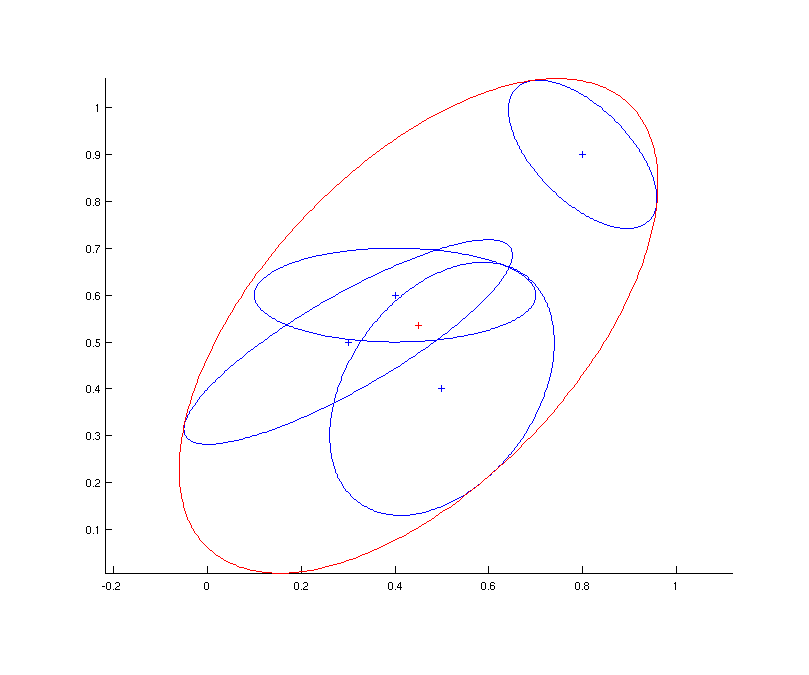
\includegraphics[width=0.6\textwidth]{figures/cu2d-4.png}
    \caption{\it 1-$\sigma$ contour ellipsoids for four inputs (blue) together with the batch Generalized CU result
        (red) for example \ref{ex:gcu2d}.}
    \label{fig:cu2d-4}
\end{figure}
\begin{equation}
    (\v{u},\m{U}) = \left(\left[
        \begin{smallmatrix}
            0.4499\\
            0.5342
        \end{smallmatrix}\right],
        \left[
        \begin{smallmatrix}
            0.2606 &  0.1559\\
            0.1559 &  0.2778
        \end{smallmatrix}\right]\right)
\end{equation}




It is next necessary to consider the ellipsoid $\varepsilon_1$ from equation
\ref{eqn:coveps} and $\tau_1(\alpha_1)$ from equation \ref{eqn:covtau}:
\begin{align}
    \varepsilon_1 &= \mathbb{T}\left(\v{m}_1,\m{M}_1\right) =
        \mathbb{T}\left(\left[\begin{smallmatrix}0.3000\\0.5000\end{smallmatrix}\right],
            \left[\begin{smallmatrix}0.1224 & 0.0650\\0.0650&0.0475\end{smallmatrix}\right]\right)\\
    \tau_1(\alpha_1) &= \mathbb{T}\left(\v{u},\frac{\m{M}_1}{\alpha_1}+\frac{(\v{u}-\v{m}_1)(\v{u}-\v{m}_1)'}{1-\alpha_1}\right)\\
        &= \mathbb{T}\left(\left[\begin{smallmatrix}0.4499\\0.5342\end{smallmatrix}\right],
        \frac{\left[\begin{smallmatrix}0.1225&0.0650\\0.0650&0.0475\end{smallmatrix}\right]}{\alpha_1}+
        \frac{\left[\begin{smallmatrix}0.0225&0.0051\\0.0051&0.0012\end{smallmatrix}\right]}{1-\alpha_1}\right).
\end{align}
From equation \ref{eqn:cu2e}, the transformation into ellipsoid space is:
\begin{align}
    \varepsilon_1 &= \left\{
        \begin{aligned}
            A_{\varepsilon,1} &= \left[\begin{smallmatrix}29.6875& -40.5949\\ -40.5949& 76.5625\end{smallmatrix}\right]\\
            b_{\varepsilon,1} &= \left[\begin{smallmatrix}11.3912\\-26.1028\end{smallmatrix}\right]\\
            c_{\varepsilon,1} &= \begin{smallmatrix}9.6340\end{smallmatrix}
        \end{aligned}\right.,\\\nonumber
    \tau_1(\alpha_1) &= \left\{
        \begin{aligned}
            A_{\tau,1} &= \left({\frac{\left[\begin{smallmatrix}0.1224 & 0.0650\\0.0650& 0.0475\end{smallmatrix}\right]}{\alpha_1}
                                  +\frac{\left[\begin{smallmatrix}0.0225 & 0.0051\\0.0051& 0.0012\end{smallmatrix}\right]}{1-\alpha_1}}\right)^{-1} \\
            b_{\tau,1} &= -\left({\frac{\left[\begin{smallmatrix}0.1224 & 0.0650\\0.0650& 0.0475\end{smallmatrix}\right]}{\alpha_1}
                                  +\frac{\left[\begin{smallmatrix}0.0225 & 0.0051\\0.0051& 0.0012\end{smallmatrix}\right]}{1-\alpha_1}}\right)^{-1} 
                          \left[\begin{smallmatrix}0.3\\0.5\end{smallmatrix}\right]\\
            c_{\tau,1} &= \left[\begin{smallmatrix}0.3&0.5\end{smallmatrix}\right] 
                            \left({\frac{\left[\begin{smallmatrix}0.1224 & 0.0650\\0.0650& 0.0475\end{smallmatrix}\right]}{\alpha_1}
                                  +\frac{\left[\begin{smallmatrix}0.0225 & 0.0051\\0.0051& 0.0012\end{smallmatrix}\right]}{1-\alpha_1}}\right)^{-1} 
                          \left[\begin{smallmatrix}0.3\\0.5\end{smallmatrix}\right] -1\\
        \end{aligned}\right.
\end{align}

\begin{figure}[tbp]
    \centering
        \subfloat[$\alpha_1$=0.05]{\label{fig:alpha2d05}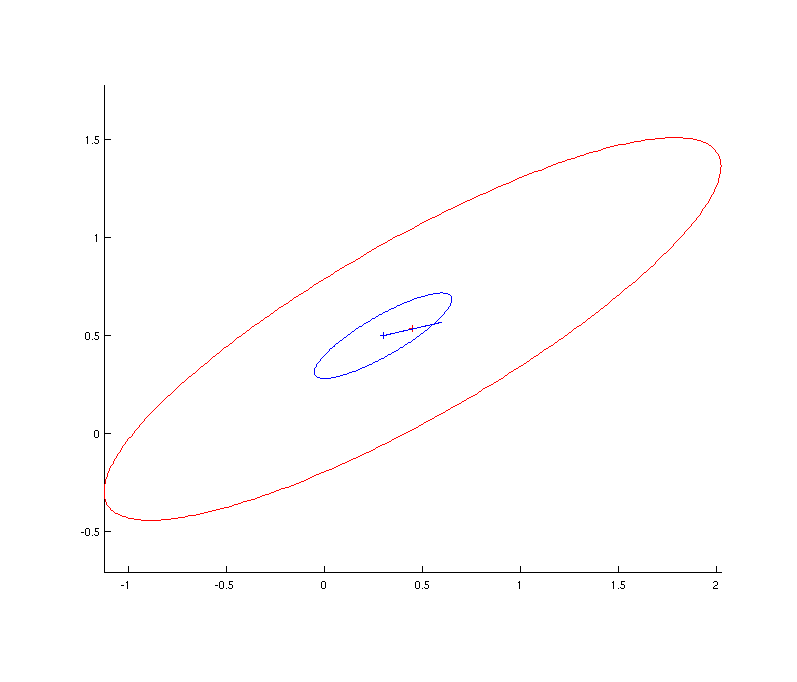
\includegraphics[width=0.4\textwidth]{figures/alpha2d-05.png}}
        \subfloat[$\alpha_1$=0.25]{\label{fig:alpha2d25}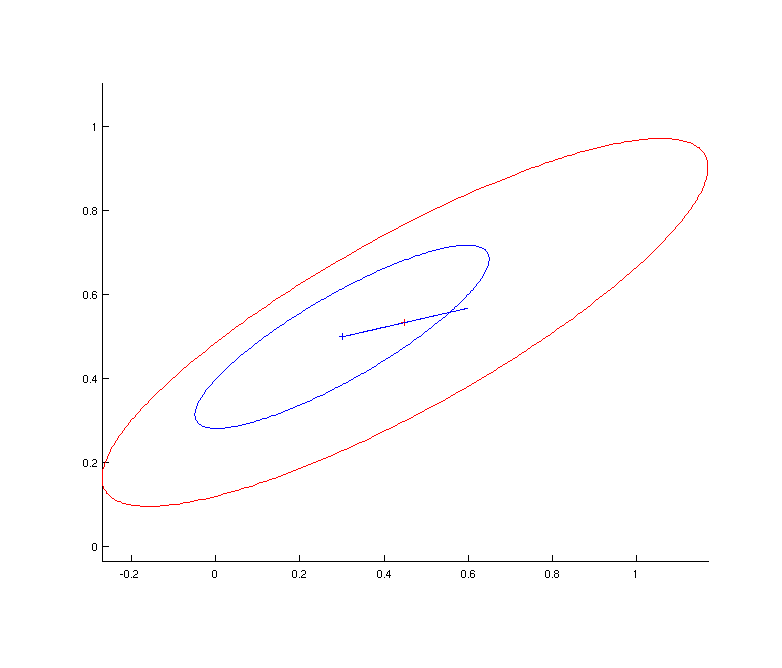
\includegraphics[width=0.4\textwidth]{figures/alpha2d-25.png}}
        \subfloat[$\alpha_1$=0.50]{\label{fig:alpha2d50}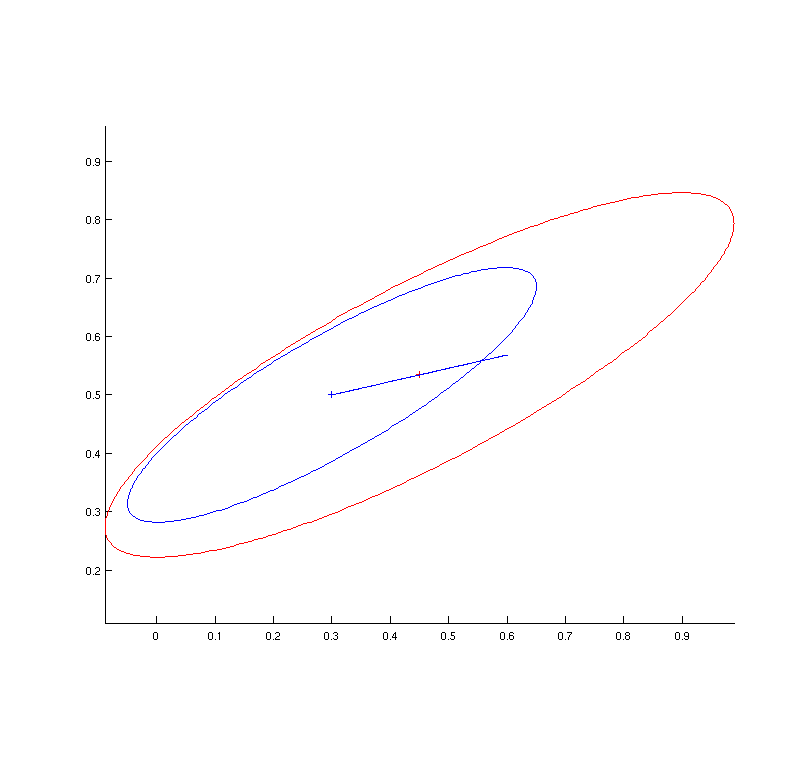
\includegraphics[width=0.4\textwidth]{figures/alpha2d-50.png}}
        \subfloat[$\alpha_1$=0.75]{\label{fig:alpha2d75}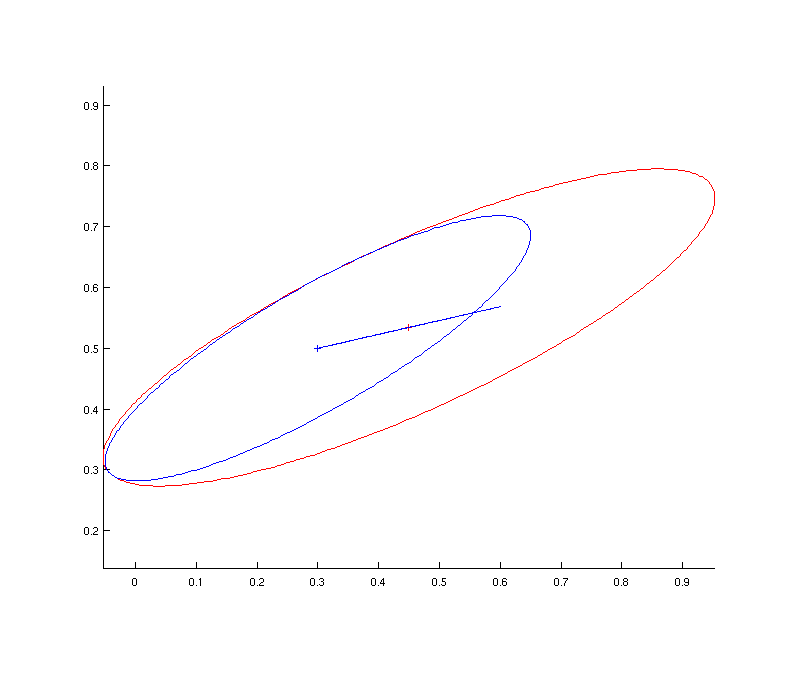
\includegraphics[width=0.4\textwidth]{figures/alpha2d-75.png}}
        \subfloat[$\alpha_1$=0.95]{\label{fig:alpha2d95}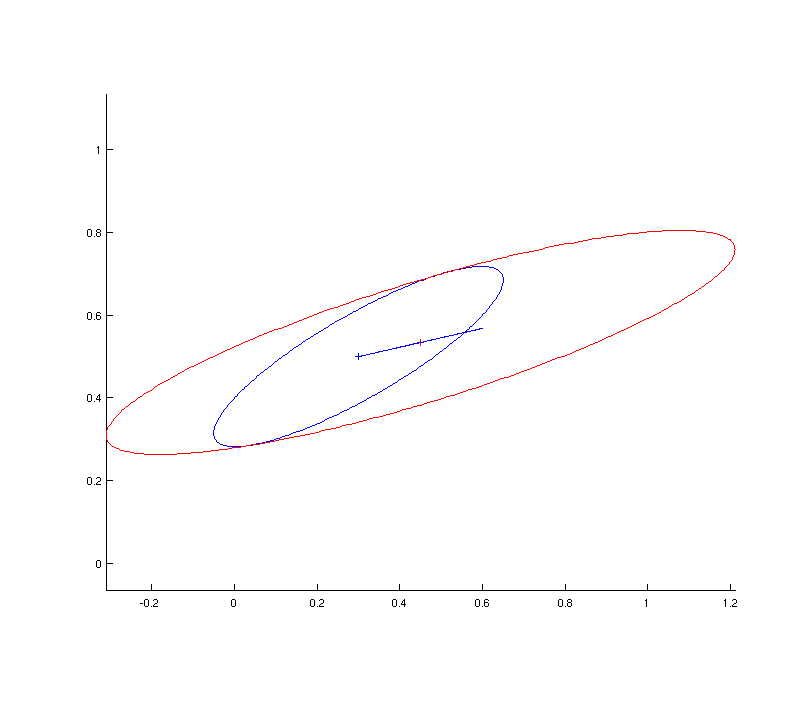
\includegraphics[width=0.4\textwidth]{figures/alpha2d-95.png}}
    \caption{\it 1-$\sigma$ contour ellipse for estimate $(\v{m}_1,\m{M}_1)$ and the mean shift term
        $(\v{u}-\v{m}_1)(\v{u}-\v{m}_1)'$ (blue), together with the intermediate covariance 1-$\sigma$ ellipse (red),
        for example \ref{ex:gcu2d}.}
    \label{fig:alpha2d}
\end{figure}
Figure \ref{fig:alpha2d} shows the 1-$\sigma$ contour ellipse of $(\v{m}_1,\m{M}_1)$ and
$\left(\v{u},\frac{\m{M}_1}{\alpha_1}+\frac{(\v{u}-\v{m}_1)(\v{u}-\v{m}_1)'}{1-\alpha_1}\right)$ for different values of
$\alpha_1$. The input $(\v{m}_1,\m{M}_1)$ is given. The mean shift term $(\v{u}-\v{m}_1)(\v{u}-\v{m}_1)'$ is a
single-component matrix which forms an ellipse with major axis twice the length of the shift, and minor axis of
length zero, centered at $\v{u}$ and aligned with both means. The intermediate covariance is a linear sum of these two
components, with the interpolation between $\alpha_1=0$ and $\alpha_1=1$ creating an unbounded asymptotic behavior which
is roughly similar to that shown in figure \ref{fig:alpha1dcurve} in the 1-D case. The 1-$\sigma$ ellipse given by
$\tau_1(\alpha_1=0)$ will be infinite in size, with the same shape as $\varepsilon_1$; at the other end,
$\tau_1(\alpha_1=1)$ will be infinite in length, with the same orientation as the mean shift term and the exact width of
the projection of $\varepsilon_1$ in the orthogonal direction.

By choosing values for $\alpha_1$ it is possible to compare $\tau_1(\alpha_1)$ with $\varepsilon_1$ and test for
containment and confirm that $\varepsilon_1$ is always completely contained. Taking $\alpha_1=0.75$, $\tau_1$ becomes
\begin{equation}
    \tau_1(\alpha_1=0.75)=\left\{
        \begin{aligned}
            A_{\tau,1} &=
            \left[\begin{smallmatrix}
                 11.8286 & -18.6285\\
                -18.6285 &  44.0408
            \end{smallmatrix}\right]\\
            b_{\tau,1} &=
            \left[\begin{smallmatrix}
                  4.6295\\
                -15.1454
            \end{smallmatrix}\right]\\
            c_{\tau,1} &=  \begin{smallmatrix}6.0078\end{smallmatrix}
        \end{aligned}\right.
\end{equation}
and the solution to $\lambda_{max}$ described in section \ref{section:containment} is $-0.0696$, so the condition
$\lambda_{max}\leq 0$ for $\tau_1$ to properly contain $\varepsilon_1$~\cite{eberly00}, holds.


\end{example}


% ND, projections
\section{Extension to Higher Dimensions}


It becomes increasingly difficult to visualize any of the covariance or ellipsoid components as the dimensionality
increases. For example, in three dimensions, the 1-$\sigma$ contour ellipsoid is a three-dimensional cross-section of a
four-dimensional Gaussian volume, which is rotated by both an elevation angle $\phi$ and an azimuth angle
$\theta$. However, even in these higher state spaces, the mathematics operate in the same fashion as described for the
one- and two-dimensional cases.

One rough method to check a higher-dimensional GCU result for ellipsoid enclosure (although not strictly {\em minimal}
enclosure) is to project the set of $n$-dimensional ellipsoids into all possible two-dimensional major axis component
planes. Properly contained ellipsoids should still be properly contained in any lower-dimensional projection. Figure
\ref{fig:cu3d} illustrates this property by projecting a set of three-dimensional 1-$\sigma$ contour ellipsoids into the
$xy$, $xz$, and $yz$ planes.
\begin{figure}[tbp]
    \centering
        \subfloat[Projection into $xy$ plane]{\label{fig:cu3dxy}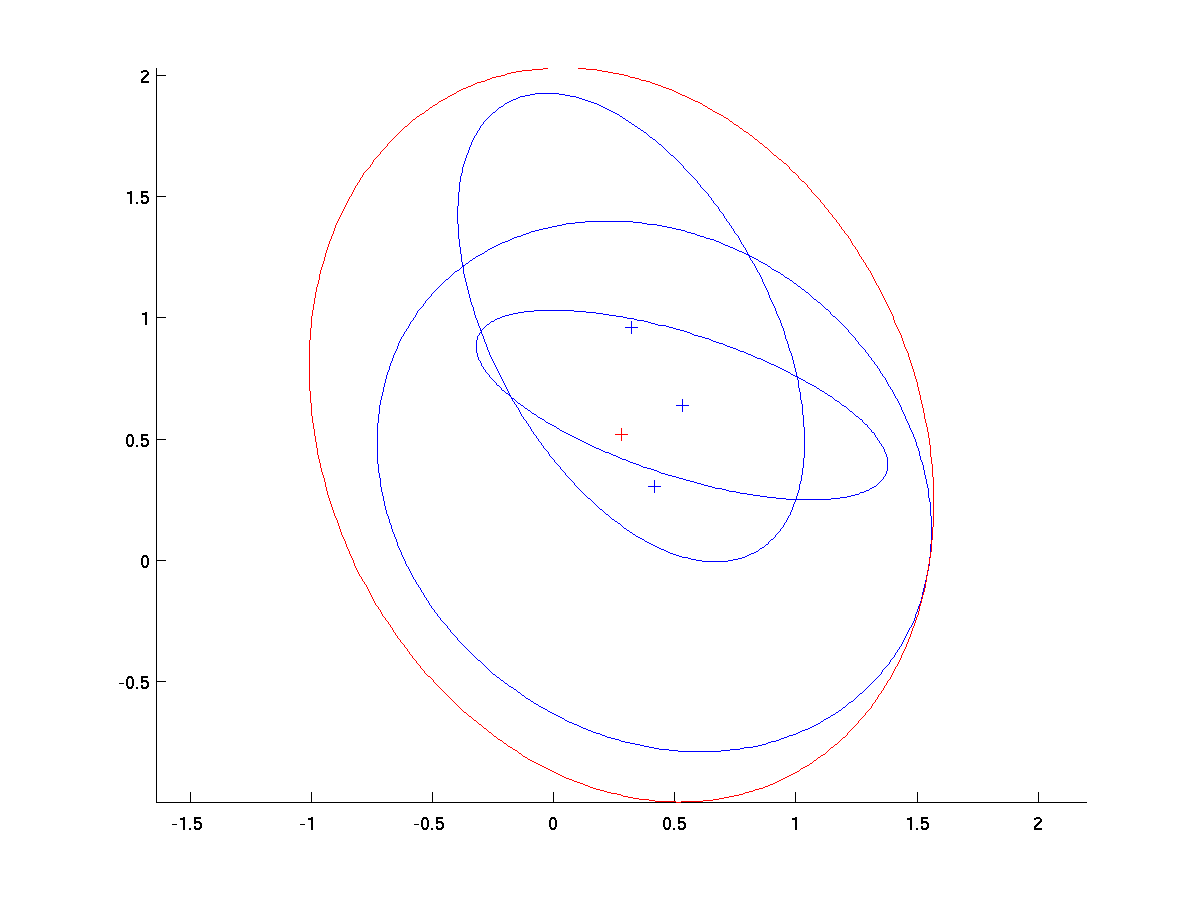
\includegraphics[width=0.4\textwidth]{figures/cu3dxy.png}}
        \subfloat[Projection into $xz$ plane]{\label{fig:cu3dxz}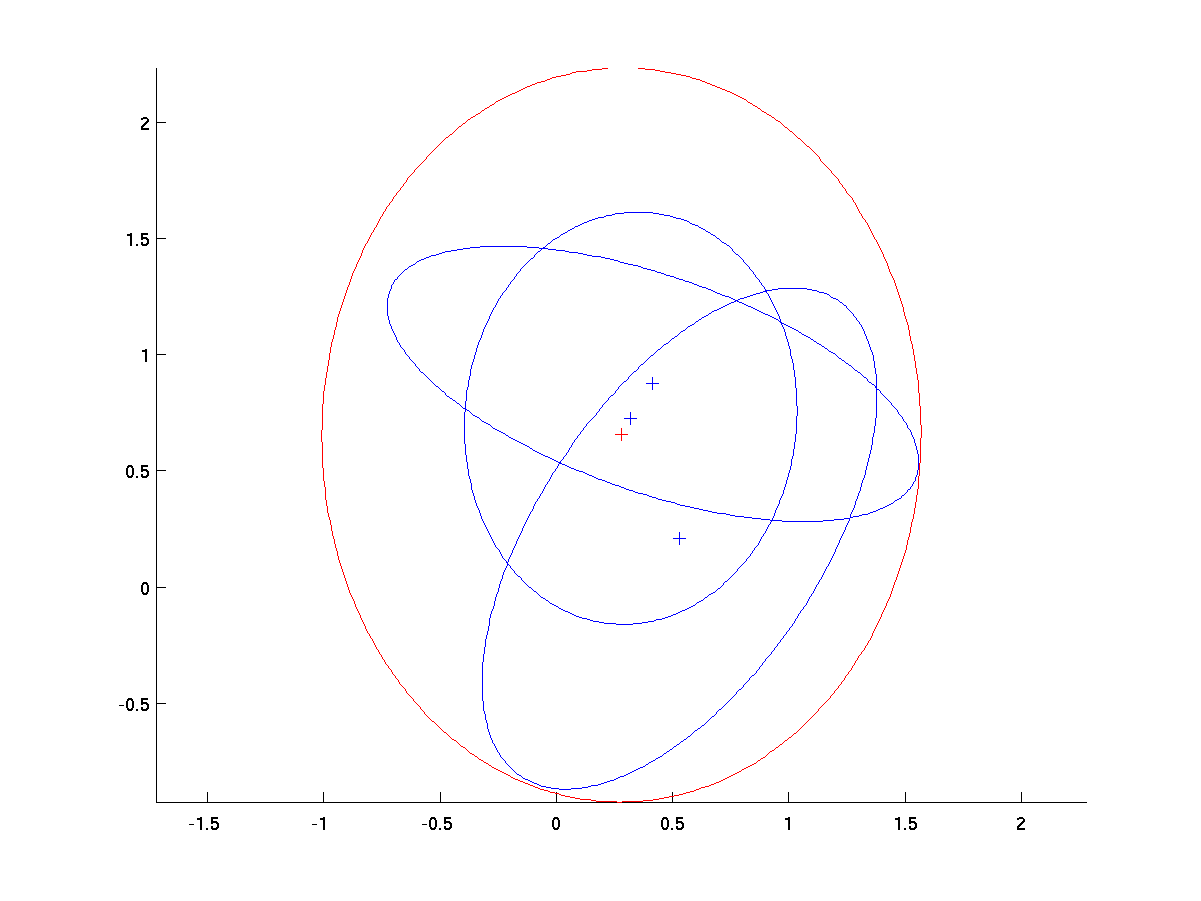
\includegraphics[width=0.4\textwidth]{figures/cu3dxz.png}}
        \subfloat[Projection into $yz$ plane]{\label{fig:cu3dyz}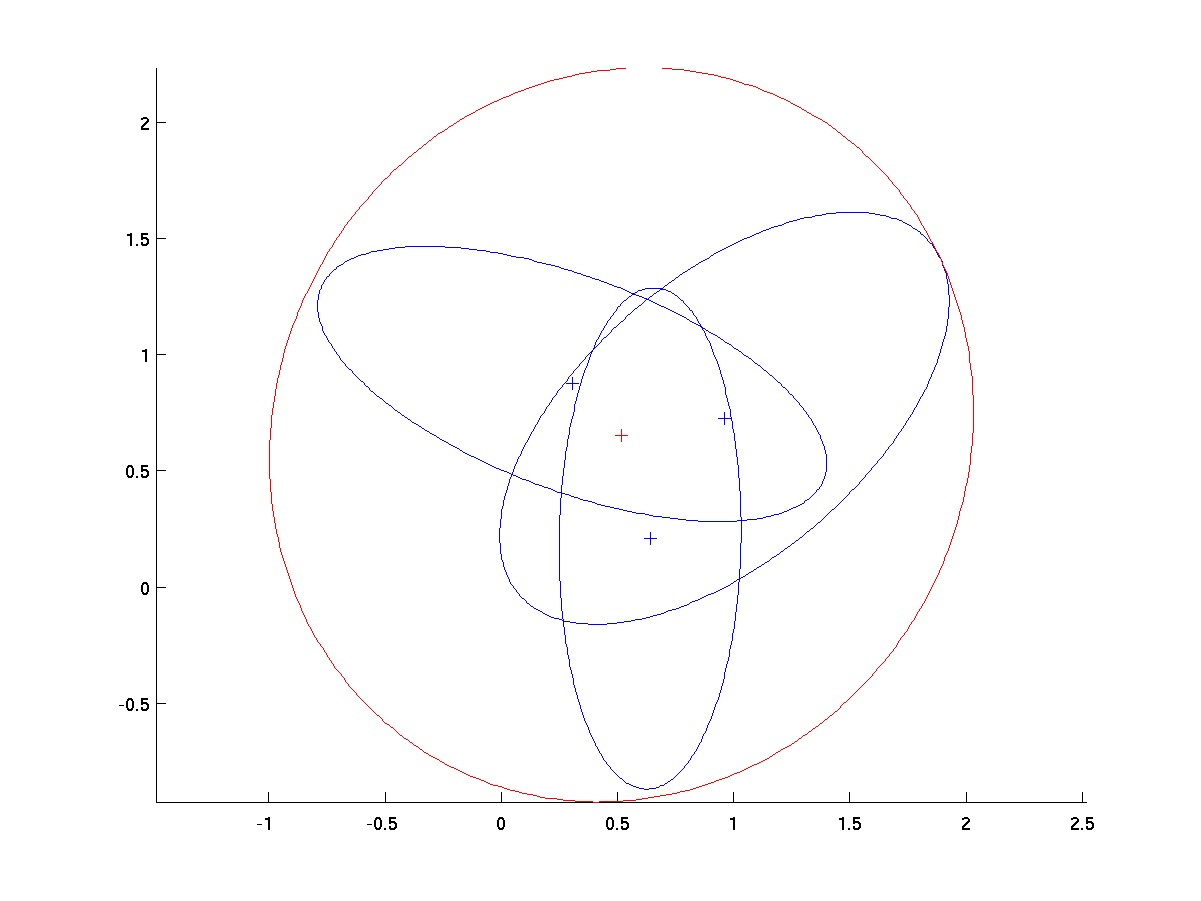
\includegraphics[width=0.4\textwidth]{figures/cu3dyz.png}}
    \caption{\it 1-$\sigma$ contour plots of three 3D input estimates (blue) together with the batch GCU result (red),
        projected down into the three 2D major axis component planes. }
    \label{fig:cu3d}
\end{figure}
Computation of the sixth-order $P(t)$ polynomial (equation \ref{eqn:poly}) for the Lagrange test confirms that the GCU
result 1-$\sigma$ contour ellipsoid properly contains its inputs in three-dimensional space as well, the space in which
this result is known to be minimized.


% Additional 2D figures
\section{Additional Examples}\label{section:examples}

In this section, further examples of two-dimensional GCU are plotted as 1-$\sigma$ contour ellipses to provide further
evidence that a GCU solution satisfies the MEEE requirements. The procedure used for each example is:
\begin{enumerate}
    \item Randomly generate five mean and covariance estimates, $(\v{m}_i,\m{M}_i)$, $i=1\dots 5$.
    \item Calculate $(\v{u},\m{U})$ as the batch GCU of $(\v{m}_i,\m{M}_i)$, $i=1\dots 5$.
    \item Use the transformation in equation \ref{eqn:cu2e} to find the ellipses $\varepsilon_0=\mathbb{T}(\v{u},\m{U})$
        and $\varepsilon_i=\mathbb{T}(\v{m}_i,\m{M}_i)$, $i=1\dots 5$.
    \item Use the procedure in section \ref{section:containment} to find $\lambda_{max}$ for each $Q_0$ and $Q_i$,
        $i=1\dots 5$.
\end{enumerate}
The fives values of $\lambda_{max}\leq 0$ are given as numerical results to support the claim that each GCU ellipse
actually does properly contain all of its inputs~\cite{eberly00}. The 1-$\sigma$ contour plots are shown in figure
\ref{fig:cu2d-5}, and the numerical values of $\lambda_{max}$ are listed in table \ref{tab:cu2d-5}.

\begin{figure}[tbp]
    \centering
        \subfloat[]{\label{fig:cu2d-5a}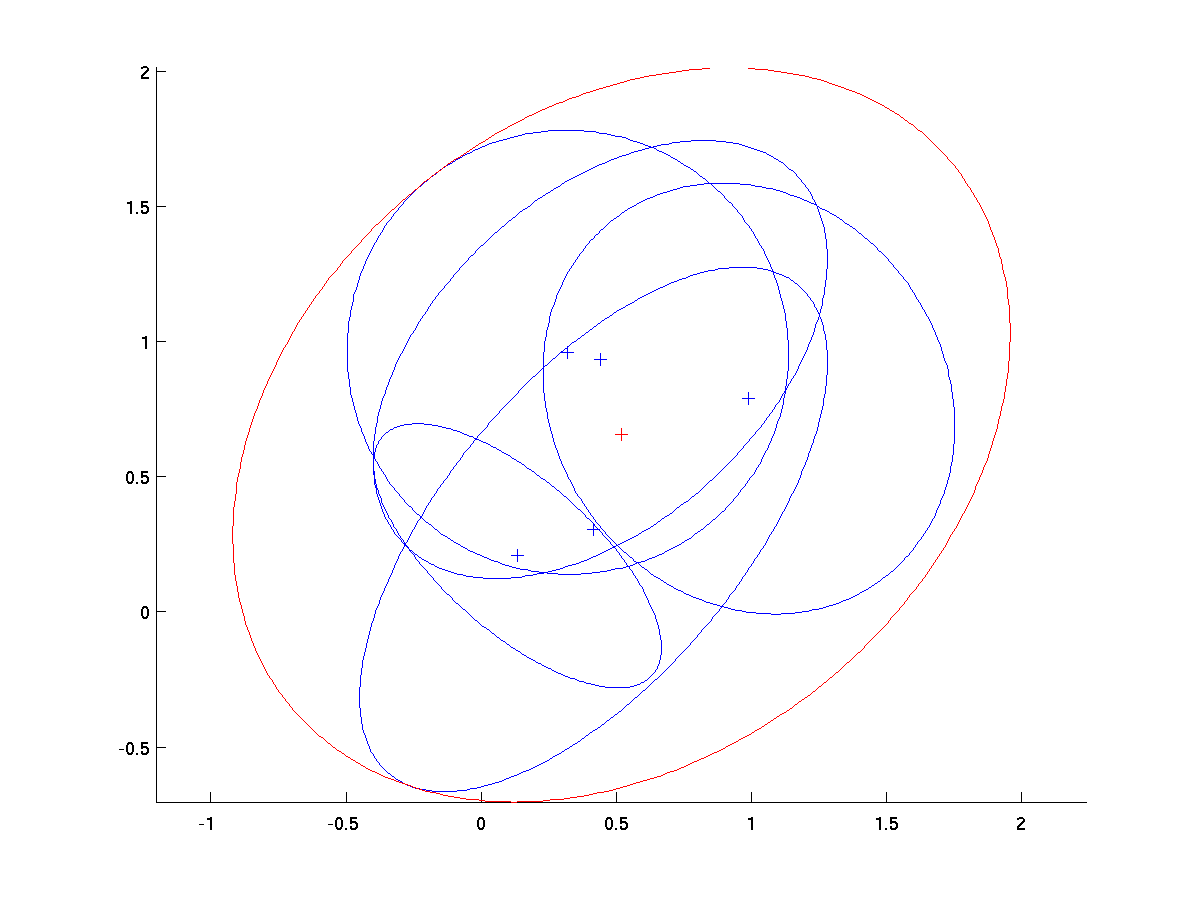
\includegraphics[width=0.4\textwidth]{figures/cu2d-5a.png}}
        \subfloat[]{\label{fig:cu2d-5b}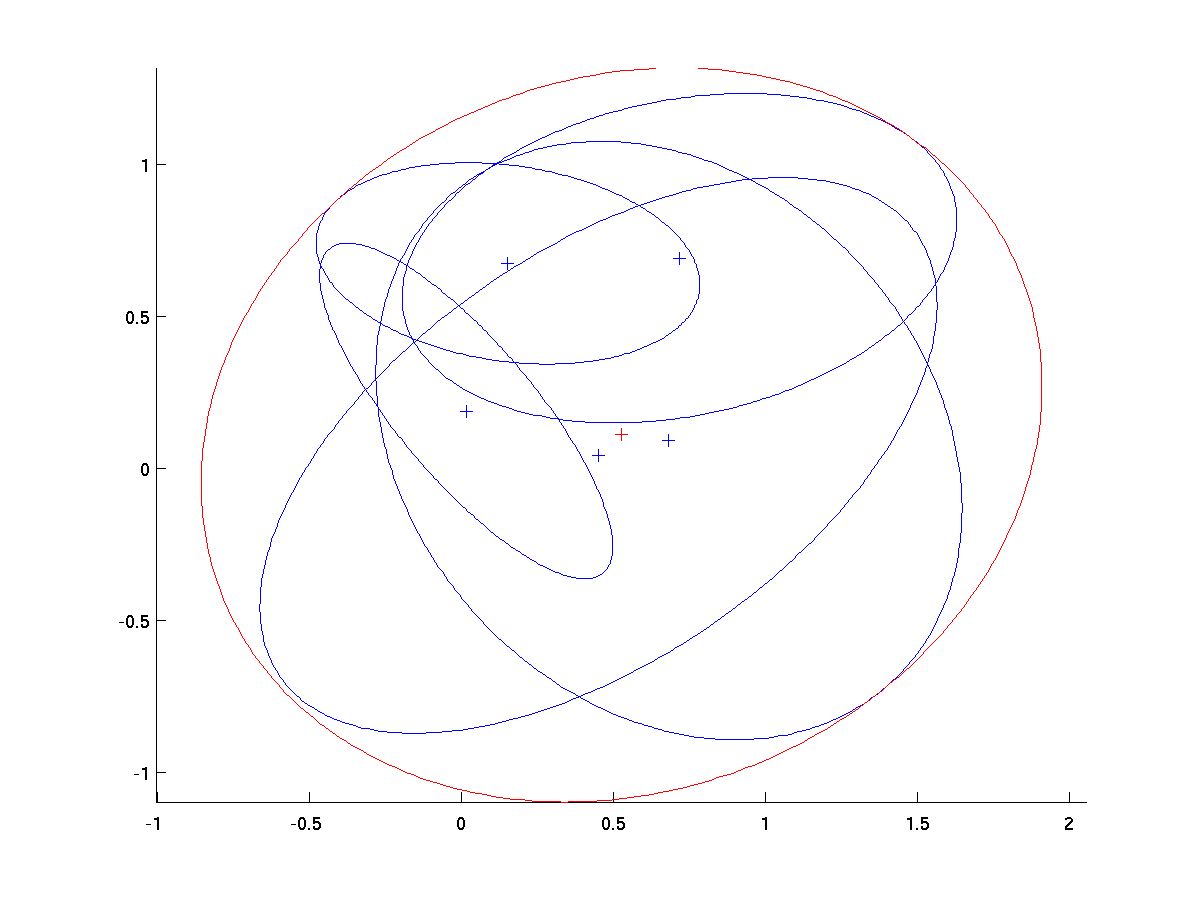
\includegraphics[width=0.4\textwidth]{figures/cu2d-5b.png}}
        \subfloat[]{\label{fig:cu2d-5c}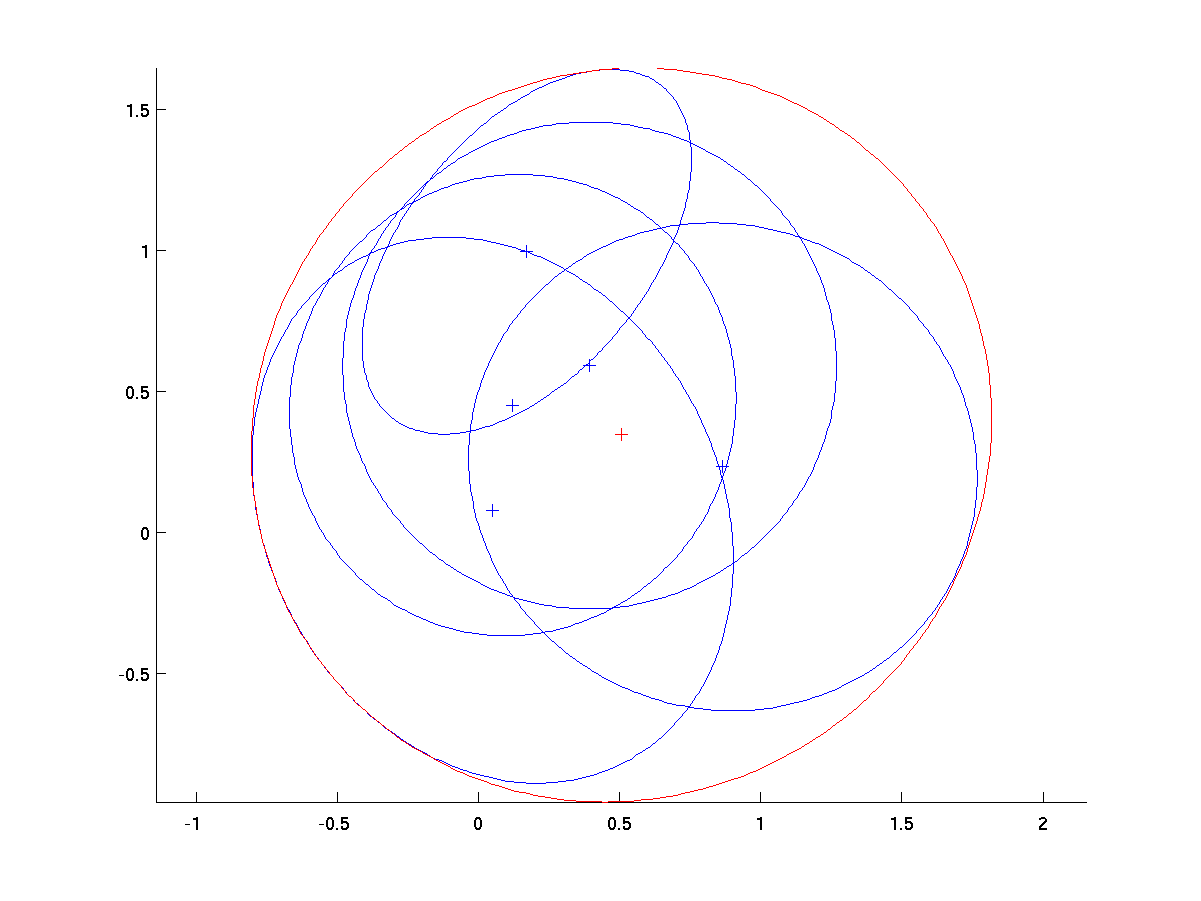
\includegraphics[width=0.4\textwidth]{figures/cu2d-5c.png}}
        \subfloat[]{\label{fig:cu2d-5d}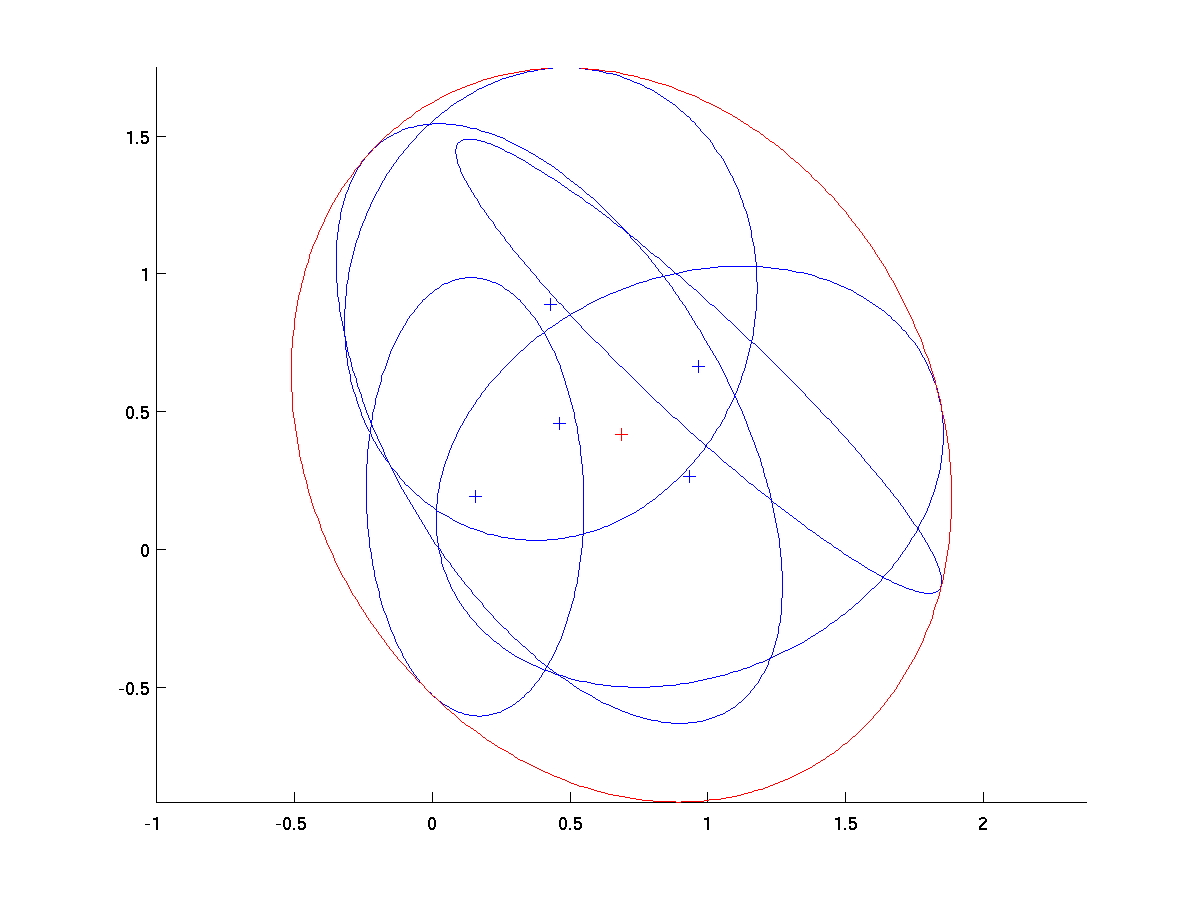
\includegraphics[width=0.4\textwidth]{figures/cu2d-5d.png}}
        \subfloat[]{\label{fig:cu2d-5e}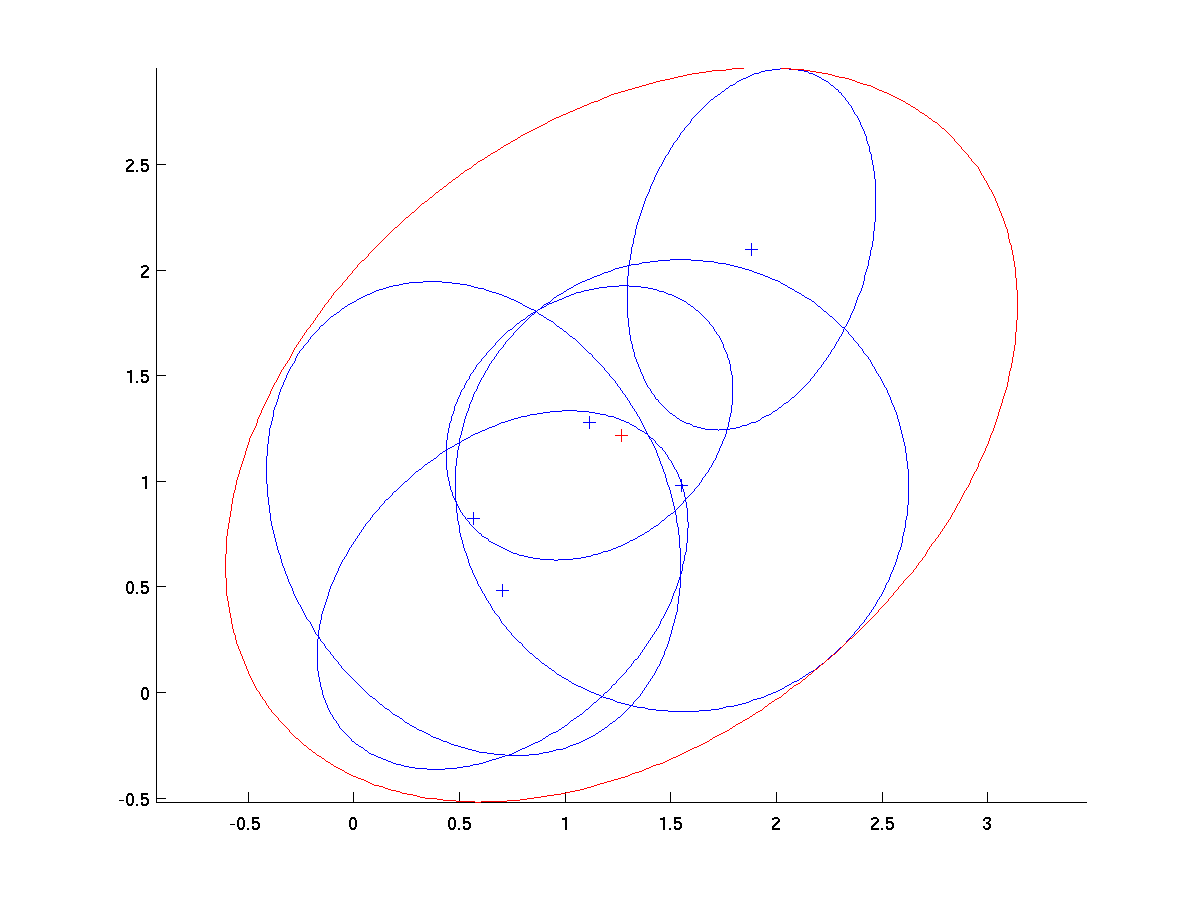
\includegraphics[width=0.4\textwidth]{figures/cu2d-5e.png}}
        \subfloat[]{\label{fig:cu2d-5f}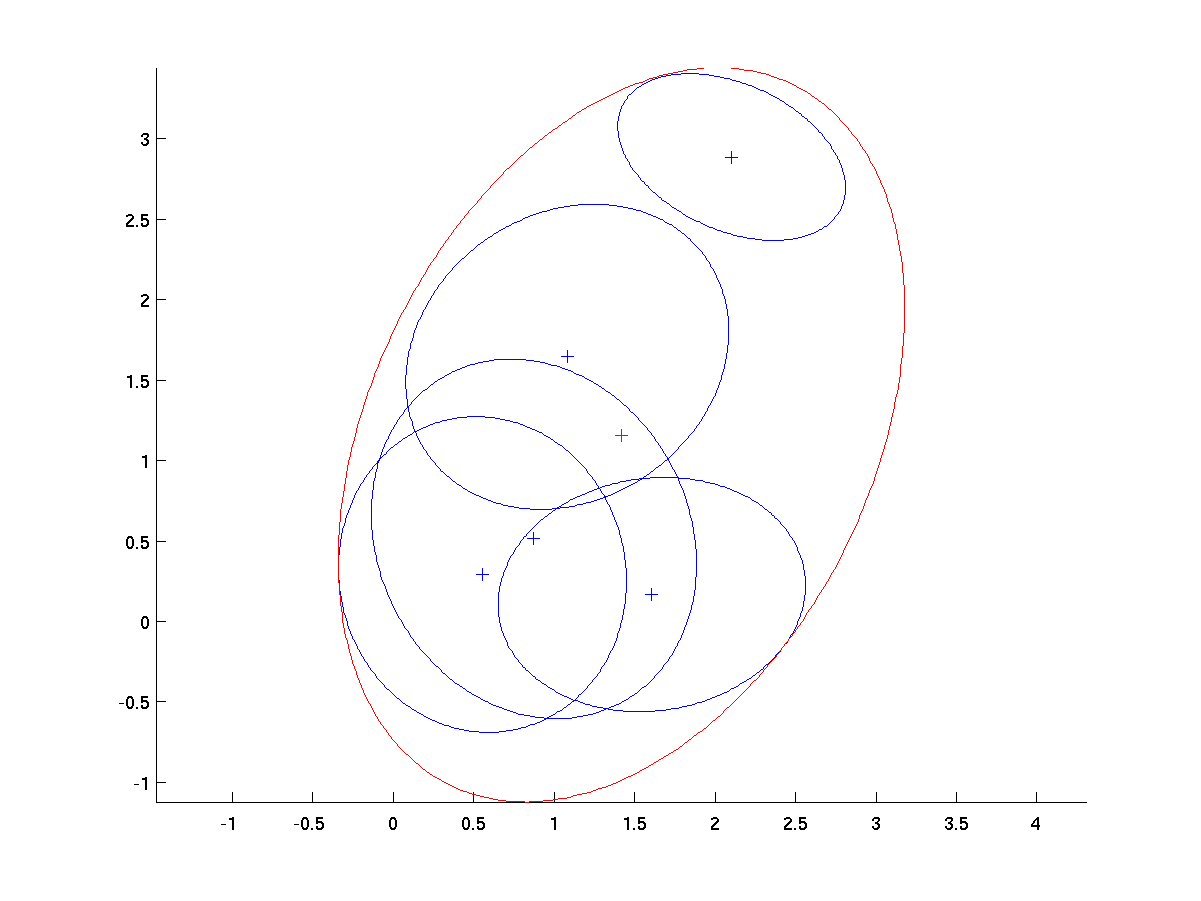
\includegraphics[width=0.4\textwidth]{figures/cu2d-5f.png}}
    \caption{\it 1-$\sigma$ contour plots of five 2D input estimates (blue) together with the batch GCU result (red). Figures
        (a) through (f) are independent examples, and the numerical results for
        $\lambda_{max}$ are given in table \ref{tab:cu2d-5}. }
    \label{fig:cu2d-5}
\end{figure}

\begin{table}
\centering
\begin{tabular*}{0.8\textwidth}{@{\extracolsep{\fill}}r@{.}lr@{.}lr@{.}lr@{.}lr@{.}lr@{.}l}
\multicolumn{2}{c}{Ex. (a)} &
\multicolumn{2}{c}{Ex. (b)} &
\multicolumn{2}{c}{Ex. (c)} &
\multicolumn{2}{c}{Ex. (d)} &
\multicolumn{2}{c}{Ex. (e)} &
\multicolumn{2}{c}{Ex. (f)}\\
\hline
-1&40e-4    &  -0&0264      &  -0&1592  &  -2&24e-5 &  -6&64e-5 &  -0&1353 \\
-0&1374     &  -2&31e-5     &  -0&0095  &  -9&24e-4 &  -0&7482  &  -0&0078 \\
-1&99e-5    &  -0&1508      &  -3&96e-5 &  -4&44e-5 &  -1&51e-4 &  -1&64e-4 \\
-0&3566     &  -1&21e-4     &  -5&16e-5 &  -1&53e-5 &  -0&1234  &  -0&2035 \\
-0&4794     &  -1&79e-4     &  -0&2109  &  -1&19e-5 &  -0&0356  &  -1&72e-5\\
\end{tabular*}
    \caption{\it Five $\lambda_{max}$ values for the six GCU trials shown in figure \ref{fig:cu2d-5}. Note that all of these
        values satisfy the condition $\lambda_{max}\leq 0$ to show that the GCU 1-$\sigma$ contour ellipse properly contains its 
        five inputs. } 
    \label{tab:cu2d-5}
\end{table}






\typeout{}
\chapter{Conclusion}\label{chapter:conclusion}

\section{Discussion}

\PARstart{T}{his thesis} has presented a technique from data fusion called Generalized Covariance Union, an important
member in the hierarchy of data fusion tools. GCU allows data fusion operations to be performed in the presence of
possibly correlated and/or spurious input, but its current implementation does not provide a real-time response in
higher-dimensional state spaces.

GCU can be graphically plotted in such a way as to suggest equivalence with the Minimal Enclosing Ellipsoid of
Ellipsoids problem, which would allow computational geometry tools to be applied to solve the GCU optimization problem.
The 1-$\sigma$ contour ellipsoids which uniquely define the Gaussian PDF associated with an error covariance, and the
covariance-to-ellipsoid transformation given in equation \ref{eqn:cu2e}, are interchangeable, and this provides a
mechanism for testing whether Generalized CU and MEEE do in fact solve the same problem. The logic outlined in section
\ref{section:explanation} and the experimental evidence illustrated in examples \ref{ex:gcu1d} and \ref{ex:gcu2d}, and
in section \ref{section:examples}, suggest that the answer to this question is yes.


\section{Future Work}

Although the experimental evidence presented is suggestive, it is not conclusive. Before research on GCU and MEEE can be
merged, there must be a rigorous proof in place showing that these two techniques are equivalent in any dimensionality.
Once this proof is established, it will be possible to solve GCU using MEEE algorithms, and vice-versa. The immediate
benefit will be a direct comparison of software running time of implementations of each technique, leading toward
improved real-time responses in both domains. Additionally, once it becomes accepted that GCU and MEEE are
interchangeable, this will allow for further investigation into other relationships between the fields of data fusion
and computational geometry. Perhaps these relationships exist not only between the two techniques used in this thesis,
but are in fact an indication of a larger degree of compatibility between two previously unrelated classes of problems.

This thesis contains the first formal analysis of GCU, following its initial presentation to the 9th International
Conference on Information Fusion in 2006, in~\cite{fusion06}. Planned future work includes a journal article covering
the GCU--MEEE equivalence. Although past and current research has been hampered by the lack of available tools---e.g. the
current implementation of CU/GCU is the first of its kind---continuing refinement to the CU/GCU optimization problem
will no doubt prove invaluable to further study, eventually leading to a robust real-time tool for mainstream data fusion
applications.





%========== Appendices==================
%\appendix

%========== Bibliography
\typeout{}
\linespread{1.0}
\setlinespacing{1.0}
\bibliography{chapters/citations.bib}
\bibliographystyle{IEEEtran}	

%========== VITA
%\typeout{}
%\linespread{1.66}
%\include{chapters/vita}
\end{document}
